% -*- Mode:TeX -*-

%% IMPORTANT: The official thesis specifications are available at:
%%            http://libraries.mit.edu/archives/thesis-specs/
%%
%%            Please verify your thesis' formatting and copyright
%%            assignment before submission.  If you notice any
%%            discrepancies between these templates and the 
%%            MIT Libraries' specs, please let us know
%%            by e-mailing thesis@mit.edu

%% The documentclass options along with the pagestyle can be used to generate
%% a technical report, a draft copy, or a regular thesis.  You may need to
%% re-specify the pagestyle after you \include  cover.tex.  For more
%% information, see the first few lines of mitthesis.cls. 

%\documentclass[12pt,vi,twoside]{mitthesis}
%%
%%  If you want your thesis copyright to you instead of MIT, use the
%%  ``vi'' option, as above.
%%
%\documentclass[12pt,twoside,leftblank]{mitthesis}
%%
%% If you want blank pages before new chapters to be labelled ``This
%% Page Intentionally Left Blank'', use the ``leftblank'' option, as
%% above. 

\documentclass[12pt,twoside]{mitthesis}

\usepackage{mathtools}

\usepackage{lgrind}
%% These have been added at the request of the MIT Libraries, because
%% some PDF conversions mess up the ligatures.  -LB, 1/22/2014
\usepackage{cmap}
\usepackage[T1]{fontenc}

% Generating the links in ToC and cite
\usepackage{hyperref}

\usepackage{tikz}
\usetikzlibrary{positioning,chains}

% plot such as sigmoid, 
\usepackage{pgfplots}
\pgfplotsset{compat=1.8}

% Originally this was the style
\pagestyle{plain}

%% This bit allows you to either specify only the files which you wish to
%% process, or `all' to process all files which you \include.
%% Krishna Sethuraman (1990).

%\typein [\files]{Enter file names to process, (chap1,chap2 ...), or `all' to
%process all files:}
\def\all{all}
%\ifx\files\all \typeout{Including all files.} \else \typeout{Including only \files.} \includeonly{\files} \fi

\usepackage{fancyhdr}
%\usepackage{acro}

%\nomenclature{$JADD$}{Joint Attention for Autonomous Driving}
\nomenclature{$GPU$}{Graphics Processing Unit}
\nomenclature{$C/NC$}{Crossing/No crossing}
\nomenclature{$SVM$}{Support Vector Machine}
\nomenclature{$CNN/ConvNet$}{Convolutional Neural Network}
\nomenclature{$DNN$}{Deep Neural Network}
\nomenclature{$RNN$}{Recurrent Neural Network}
\nomenclature{$AI$}{Artificial Intelligence}
\nomenclature{$R-CNN$}{Region-Convolutional Neural Network}
\nomenclature{$SSD$}{Single Shot Detection}
\nomenclature{$IoU$}{Intersection over Union}
\nomenclature{$ADAS$}{Advanced driver-assistance systems}










\usepackage{nomencl}
\makenomenclature
 
\renewcommand{\nomname}{Abbreviation}

\begin{document}


\title{Deep Learning: Pedestrian trajectory detection}

\author{Kalinga Bhusan Ray}

\department{Fakult{\"a}t f{\"u}r Informatik und Automatisierung}

\degree{Master of Science (M. Sc.) in  Research in Computer \& Systems Engineering}

%\newcommand{\artderausarbeitung}{Bachelorarbeit}
%\newcommand{\namedesautors}{Max Mustermann}
%\newcommand{\themaderarbeit}{Anfertigung einer Ausarbeitung mit \LaTeX}

% PDF Metadaten definieren
%\hypersetup{
%   pdftitle={\themaderarbeit},
%   pdfsubject={\artderausarbeitung},
%   pdfauthor={\namedesautors},
%   pdfkeywords={\artderausarbeitung; TU-Ilmenau; Kommunikationsnetze;}}
	
% As of the 2007-08 academic year, valid degree months are September, 
% February, or June.  The default is June.
\degreemonth{Oct}
\degreeyear{2019}
\thesisdate{Oct 15, 2019}

%% By default, the thesis will be copyrighted to MIT.  If you need to copyright
%% the thesis to yourself, just specify the `vi' documentclass option.  If for
%% some reason you want to exactly specify the copyright notice text, you can
%% use the \copyrightnoticetext command.  
%\copyrightnoticetext{\copyright IBM, 1990.  Do not open till Xmas.}

% If there is more than one supervisor, use the \supervisor command
% once for each.
\supervisor{Prof. Dr.-Ing. habil. Pu Li}{University Professor}

% This is the department committee chairman, not the thesis committee
% chairman.  You should replace this with your Department's Committee
% Chairman.
\chairman{Prof. Dr.-Ing. habil. Andreas Mitschele-Thiel}{Chairman, examination committee}

% Make the titlepage based on the above information.  If you need
% something special and can't use the standard form, you can specify
% the exact text of the titlepage yourself.  Put it in a titlepage
% environment and leave blank lines where you want vertical space.
% The spaces will be adjusted to fill the entire page.  The dotted
% lines for the signatures are made with the \signature command.
\maketitle

% The abstractpage environment sets up everything on the page except
% the text itself.  The title and other header material are put at the
% top of the page, and the supervisors are listed at the bottom.  A
% new page is begun both before and after.  Of course, an abstract may
% be more than one page itself.  If you need more control over the
% format of the page, you can use the abstract environment, which puts
% the word "Abstract" at the beginning and single spaces its text.

%% You can either \input (*not* \include) your abstract file, or you can put
%% the text of the abstract directly between the \begin{abstractpage} and
%% \end{abstractpage} commands.

% First copy: start a new page, and save the page number.
\cleardoublepage
% Uncomment the next line if you do NOT want a page number on your
% abstract and acknowledgments pages.
% \pagestyle{empty}
\setcounter{savepage}{\thepage}
\begin{abstractpage}
% $Log: abstract.tex,v $
% Revision 1.1  93/05/14  14:56:25  starflt
% Initial revision
% 
% Revision 1.1  90/05/04  10:41:01  lwvanels
% Initial revision
% 
%
%% The text of your abstract and nothing else (other than comments) goes here.
%% It will be single-spaced and the rest of the text that is supposed to go on
%% the abstract page will be generated by the abstractpage environment.  This
%% file should be \input (not \include 'd) from cover.tex.
\begin{flushleft}
In the recent times, Deep Learning plays a significant role in the computer vision
related tasks and Deep learning based algorithms such as 'Convolutional Neural Networks'
(CNN) demonstrated and proven to be outperforming other state-of-art models when 
deployed in object detection tasks. In the recent past many researchers shown great 
deals towards image classification and object detection problems. Also there exists several 
benchmarks in the context of classification and objects in an image detection. In 
comparison usage of deep learning to solve problems that involves prediction of 
user behavior from a monitored video is much less investigated.
\vskip 1\baselineskip
\par
During my Master Thesis, various aspects related to image classification, object 
in image detection and object tracking in a video and prediction of user behavior 
have been studied with a particular focus on Pedestrian trajectory prediction. 
A new prediction model is proposed and the results for pedestrian trajectory 
task are presented.
\vskip 1\baselineskip
\textit{Keywords: image classification, object detection, object tracking, trajectory prediction}
\end{flushleft}
\end{abstractpage}

% Additional copy: start a new page, and reset the page number.  This way,
% the second copy of the abstract is not counted as separate pages.
% Uncomment the next 6 lines if you need two copies of the abstract
% page.
% \setcounter{page}{\thesavepage}
% \begin{abstractpage}
% % $Log: abstract.tex,v $
% Revision 1.1  93/05/14  14:56:25  starflt
% Initial revision
% 
% Revision 1.1  90/05/04  10:41:01  lwvanels
% Initial revision
% 
%
%% The text of your abstract and nothing else (other than comments) goes here.
%% It will be single-spaced and the rest of the text that is supposed to go on
%% the abstract page will be generated by the abstractpage environment.  This
%% file should be \input (not \include 'd) from cover.tex.
\begin{flushleft}
In the recent times, Deep Learning plays a significant role in the computer vision
related tasks and Deep learning based algorithms such as 'Convolutional Neural Networks'
(CNN) demonstrated and proven to be outperforming other state-of-art models when 
deployed in object detection tasks. In the recent past many researchers shown great 
deals towards image classification and object detection problems. Also there exists several 
benchmarks in the context of classification and objects in an image detection. In 
comparison usage of deep learning to solve problems that involves prediction of 
user behavior from a monitored video is much less investigated.
\vskip 1\baselineskip
\par
During my Master Thesis, various aspects related to image classification, object 
in image detection and object tracking in a video and prediction of user behavior 
have been studied with a particular focus on Pedestrian trajectory prediction. 
A new prediction model is proposed and the results for pedestrian trajectory 
task are presented.
\vskip 1\baselineskip
\textit{Keywords: image classification, object detection, object tracking, trajectory prediction}
\end{flushleft}
% \end{abstractpage}

\cleardoublepage

\section*{Acknowledgments}
\begin{flushleft}
Countless thanks to my parents, in-laws and relatives, especially to my wife
for giving me unfailing support and continuous encouragement throughout my 
years of study and while writing this thesis. This accomplishment would not 
have been possible without them I would like to dedicate this work to my 
grandfather Sri Baishnab Charan Mohanty who believed in me all the times
and blessed me.
\vskip 1\baselineskip
%\par
My special thanks to my supervisor Qais Mohammed Ali Yousef for his valuable
inputs, support and inspirations. He believed in me and helped me a lot.
The door to his office was always accessible whenever I had a question 
or ran into some trouble. He always enabled this Thesis to be my own work 
but did not shy away from steering me in the right direction whenever deemed necessary.
\vskip 1\baselineskip
\par
Many thanks to Prof. Dr. Pu Li, his Control Engineering course was a 
catalyst for me doing my research. Also many thanks to SOP department for 
enabling a great working environment. Special thanks to Bj{\"o}rn T{\"o}pper, 
he helped me a lot in bringing the required system and administration.
\vskip 1\baselineskip
\par
My deeply thanks to all the Professor and teaching staffs of Research 
in Computer \& Systems Engineering (RCSE) course, it was a pleasant and life 
time experience studying this course at Technische Universit{\"a}t Ilmenau.
\vskip 1\baselineskip
\par
Author
Kalinga Bhusan Ray
\end{flushleft}

%%%%%%%%%%%%%%%%%%%%%%%%%%%%%%%%%%%%%%%%%%%%%%%%%%%%%%%%%%%%%%%%%%%%%%
% -*-latex-*-


% Some departments (e.g. 5) require an additional signature page.  See
% signature.tex for more information and uncomment the following line if
% applicable.
% % -*- Mode:TeX -*-
%
% Some departments (e.g. Chemistry) require an additional cover page
% with signatures of the thesis committee.  Please check with your
% thesis advisor or other appropriate person to determine if such a 
% page is required for your thesis.  
%
% If you choose not to use the "titlepage" environment, a \newpage
% commands, and several \vspace{\fill} commands may be necessary to
% achieve the required spacing.  The \signature command is defined in
% the "mitthesis" class
%
% The following sample appears courtesy of Ben Kaduk <kaduk@mit.edu> and
% was used in his June 2012 doctoral thesis in Chemistry. 

\begin{titlepage}
\begin{large}
This doctoral thesis has been examined by a Committee of the Department
of Chemistry as follows:

\signature{Professor Jianshu Cao}{Chairman, Thesis Committee \\
   Professor of Chemistry}

\signature{Professor Troy Van Voorhis}{Thesis Supervisor \\
   Associate Professor of Chemistry}

\signature{Professor Robert W. Field}{Member, Thesis Committee \\
   Haslam and Dewey Professor of Chemistry}
\end{large}
\end{titlepage}



% Original pagestyle
\pagestyle{plain}

  % -*- Mode:TeX -*-
%% This file simply contains the commands that actually generate the table of
%% contents and lists of figures and tables.  You can omit any or all of
%% these files by simply taking out the appropriate command.  For more
%% information on these files, see appendix C.3.3 of the LaTeX manual. 
\pagenumbering{roman}
\setcounter{page}{1}
\tableofcontents
\newpage
\listoffigures
\newpage
\listoftables


\newcommand{\newpara}{\vspace{1em}\noindent}

\nomenclature{$JADD$}{Joint Attention for Autonomous Driving}
\nomenclature{$GPU$}{Graphics Processing Unit}
\nomenclature{$C/NC$}{Crossing/No crossing}
\nomenclature{$SVM$}{Support Vector Machine}
\nomenclature{$CNN/ConvNet$}{Convolutional Neural Network}
\nomenclature{$DNN$}{Deep Neural Network}
\nomenclature{$RNN$}{Recurrent Neural Network}
\nomenclature{$AI$}{Artificial Intelligence}
\nomenclature{$R-CNN$}{Region-Convolutional Neural Network}
\nomenclature{$SSD$}{Single Shot Detection}
\nomenclature{$IoU$}{Intersection over Union}
\nomenclature{$ADAS$}{Advanced driver-assistance systems}










% C:\Users\kara9147\Documents\GitHub\ML\Documents\latex>
%makeindex -s nomencl.ist -t  main.nlg -o %main.nls main.nlo
\printnomenclature

%% This is an example first chapter.  You should put chapter/appendix that you
%% write into a separate file, and add a line \include{yourfilename} to
%% main.tex, where `yourfilename.tex' is the name of the chapter/appendix file.
%% You can process specific files by typing their names in at the 
%% \files=
%% prompt when you run the file main.tex through LaTeX.
\chapter{Introduction}
\section{Motivation}
Deep Learning has made some significant impacts in the areas of image classification, 
object detection, speech recognition, text-to-speech generation, machine translation,
online recommender system, medical diagnosis and few more. With availability of high 
computing power such as high speed CPU and high bandwidth GPU, large amount of 
data from which actionable insight is expected and nice and powerful ecosystem of  
tools such as TensorFlow and PyTorch; many researchers in the scientific community 
starting from neurologist to computer scientist are enticed towards research in the area 
of Artificial Intelligence. Several interesting findings, new algorithms, record 
breaking benchmarking results while applying Deep Learning algorithms has taken 
AI to a different level.

\vspace{1em}
\noindent Unlike human, recognizing and localizing objects still remains a challenge for artificial 
systems, mainly because of two factors - view point dependent object variability and
high in-class variability. In the human detection task intra-class variability includes
color of the clothing, type of clothing, appearance, pose, illumination, partial occlusions
and background. Pedestrian detection has remain most studied problem in the computer vision.
In the last decade with application of CNNs researchers are able to get some nice results 
those are good enough for application in practical scenarios.

\vspace{1em}
\noindent The detection of the human is a partial task where human and machine must interact 
with each other and machine expected to understand human intention. For example, 
a self driving must anticipate and predict the pedestrian in a reliable manner, whether 
the pedestrian intents to cross the road, or standing near the curb or waiting at waiting shelter.
Such intent prediction problem can be viewed as two step related problem. First detect the 
human and track the person in several frames and predict after tracking for certain time using a 
previously trained model for such intention prediction.

\vspace{1em}
\noindent The main idea of this thesis is to take a look at different aspect of solving such a problem, 
starting with reliable data \footnote{There are several image and video datasets exist in the 
public domain for research purpose} acquisition, understanding the annotation in the data, 
training a neural network using efficient features for the detection of person. Detecting the same person in the series of subsequent frames and finally prediction of pedestrian intention using another classifier.

\section{Problem Statement} 
Which model to be used for the first part of the problem, which deals with detecting the pedestrians in the scene? If the model capable of detecting multiple pedestrians in the scene? What is the processing time, if the processing time under a threshold for the purpose of using it in the real time scenario?
Which kind of algorithm to use used for second part of the problem, which deals with predicting the pedestrian intention? What is the time delay of such models if such model can be applicable in real time application scenarios?
How to choose right network for such problems, training them on large dataset which includes several thousand of images or hours of real video recordings? How to set and tune several hyper parameters while training the neural network? This Thesis work mainly answers above question by investigating and  applying several methodologies into practice.

\section{Objectives}
The main idea of this thesis is establishing a Pipeline by selecting appropriate models at both stages and evaluating the end results. Acquiring the public dataset related to pedestrian movement and validating the proposed model on them and estimating the performance in accordance with the dataset owner specification for doing so.

\section{Overview}
The texts in this thesis is split as below.
\begin{itemize}
  \item {\textbf {\textit{Chapter 2}} describes CNN for feature extraction, Deep Learning, state of the art}
  \item {\textbf {\textit{Chapter 3}} explains methodology choosing right algorithm}
	\item {\textbf {\textit{Chapter 4}} presents implementation, and shows the results of various experiments and setups  }
	\item {\textbf {\textit{Chapter 5}} concludes my thesis with a summary of the main results and brief discussion for probable future topics of research}
\end{itemize}

\section{Terminology}
In the current work and by other authors also training and learning is used interchangeably. Let me loosely define some frequently used terms and concepts in the Machine Learning arena.
\\*\textbf{Epoch:}
During the learning the network sees the set of samples several times. During the training, presenting the network entire set of sample once is known as an epoch. So an epoch represents one iteration over entire dataset.
\\*\textbf{Batch and batch size:}
Mainly because of two reasons we can not pass the entire dataset to the network for the training purpose at once. Firstly, datasets by nature most of the time are huge. Let it be image data or some other textual data, in many scenarios it is not possible to feed all the data because of hardware constraints, such as not enough RAM to hold entire dataset.
Secondly to update weight during training process, network has to wait for a very very long time to calculate the delta weight after processing all the input data. To solve this problem usually the full dataset is split into several small batches and number of samples within each small batch is known as 
Batch and batch size.
\\*\textbf{Iterations:} 
Number of batches that a neural network process to complete a single epoch.
The number of  iterations, batch size and  number of data samples in the dataset is given by, the below expression.
\begin{equation}
    D = B * I
\end{equation}
Where D is the total number of samples in the dataset.
\\*B is the number of samples in the mini batch that is fed to the network at once.
\\*I is the  total number of batches the network process in a single epoch.

Larger batch size requires more computational resource and achieves faster completion, in contrast smaller batch size leads to more generalization. In this regards, Yann  LeCun humorously said
\begin{quote}
``Training with large mini batches is bad for your health. More importantly, it's bad for your test error.  Friends, don't let friends use mini batches larger than 32.''
\end{quote}   
The empirical study of the performance of mini-batch stochastic gradient descent in \cite{masters2018revisiting} show that, the team obtained the best training stability and generalization performance using small batch sizes, for a given computational cost, across a wide range of experiments they conducted. In all cases they have achieved the best results with batch sizes m = 32 or smaller.


%optimizations are described in detail in section~\ref{ch1:opts}.

%\section{Description of micro-optimization}\label{ch1:opts}

%multiplies\footnote{Using unnormalized numbers for math is not a new idea; a

%unnormalized arithmetic, with a separate {\tt NORMALIZE} instruction.}.

% This is an example of how you would use tgrind to include an example
% of source code; it is commented out in this template since the code
% example file does not exist.  To use it, you need to remove the '%' on the
% beginning of the line, and insert your own information in the call.
%
%\tagrind[htbp]{code/pmn.s.tex}{Post Multiply Normalization}{opt:pmn}


\subsection{Block Exponent}

In a unoptimized sequence of additions, the sequence of operations is as
follows for each pair of numbers ($m_1$,$e_1$) and ($m_2$,$e_2$).
\begin{enumerate}
  \item Compare $e_1$ and $e_2$.
  \item Shift the mantissa associated with the smaller exponent $|e_1-e_2|$
        places to the right.
  \item Add $m_1$ and $m_2$.
  \item Find the first one in the resulting mantissa.
  \item Shift the resulting mantissa so that normalized
  \item Adjust the exponent accordingly.
\end{enumerate}


\begin{eqnarray*}
a_i & = & a_j + a_k \\
a_i & = & 2a_j + a_k \\
a_i & = & 4a_j + a_k \\
a_i & = & 8a_j + a_k \\
a_i & = & a_j - a_k \\
a_i & = & a_j \ll m \mbox{shift}
\end{eqnarray*}
instead of the multiplication.  For example, to multiply $s$ by 10 and store
the result in $r$, you could use:
\begin{eqnarray*}
r & = & 4s + s\\
r & = & r + r
\end{eqnarray*}
Or by 59:
\begin{eqnarray*}
t & = & 2s + s \\
r & = & 2t + s \\
r & = & 8r + t
\end{eqnarray*}

{\em might\/} 

Challenges are there while just considering image data, 
the verities of image sources for example we can get photos that are taken by 
professionals, synthetic photos drawn by image generators and real life photos 
that we see and capture in our day to day life. So the results of these benchmarks and 
observation across these aforementioned classes of data set does not transfer to the other scenarios.
%% This is an example first chapter.  You should put chapter/appendix that you
%% write into a separate file, and add a line \include{yourfilename} to
%% main.tex, where `yourfilename.tex' is the name of the chapter/appendix file.
%% You can process specific files by typing their names in at the 
%% \files=
%% prompt when you run the file main.tex through LaTeX.
\chapter{State of the Art}
% object detection, pedestrain detection
%\cite{felzenszwalb2009object, walk2010new, liu2016ssd, szegedy2014scalable, dollar2009pedestrian, dollar2011pedestrian}

% feature extraction
%\cite{dalal2005histograms, lowe2004distinctive}

% Region Proposal
%\cite{girshick2014rich, girshick2015fast, ren2015faster}

% Trackers
%\cite{fiaz2019handcrafted,xu2005pedestrian,ning2017spatially}

% Activity prediction
%\cite{ryoo2011human, richard2017weakly }


% Intention prediction
%\cite{saleh2017intent, fang2018pedestrian, abu2018will, dollar2005behavior, cao2017realtime, rasouli2017agreeing }

% Trajectory prediction
%\cite{saleh2017intent, zhang2019sr, xue2018ss, lipton2015critical}

The problem of human action classification or pedestrian intent prediction, pedestrian future trajectory estimation \cite{saleh2017intent, fang2018pedestrian, abu2018will, dollar2005behavior, rasouli2017agreeing, cao2017realtime} from a sequence of images has got huge attention from the researchers in recent years. This problem is inherently complex as it is based on other complex problems. To predict future location, detect the action or intention one must first detect the object in an image and classify it, track the same object over several continuous frames. Before the dominance of the convolutional neural network (CNN) and Deep Learning which has outperformed other traditional methods in recent times. For any such prediction task, we need an efficient and robust object detection, object localization and object tracking model working seamlessly together to enable the last phase of the prediction task. Object detection and localization constitute the backbone of this pipeline and takes maximum share of the run time in the entire pipeline. To build a real-time pedestrian future bounding box prediction pipeline, it is of utmost important to find a model that performs real-time object detection \cite{felzenszwalb2009object, walk2010new, liu2016ssd, szegedy2014scalable, dollar2009pedestrian, dollar2011pedestrian} and localization reliably. In this chapter, some of the state-of-the-art models for such tasks are explored.

\section{Pedestrian intention on roads}
\newpara Abu Farha and the team presented \cite{abu2018will}, where they discussed methods to predict actions that are in a considerable future and their duration. And they tried to anticipate all activities within a horizon of 5 minutes. After inferring the activities from the observed part of the video using an RNN-HMM \cite{richard2017weakly}, they proposed two approaches to predict the future actions and their durations, in the first approach they used RNN, where the anticipated activities are fed to the RNN to predict the remaining duration of the ongoing activities and duration of the next activity along with its class.
In the second approach, the proposed CNN based single-pass model which predicts the length and label of the future action. They have found that both approaches have outperformed both the grammar-based baseline and the nearest neighbor baseline. RNN and CNN found to be performing similarly for time horizon more than 40 seconds and RNN performs better for lesser than 20 seconds time horizon. The task is more formally defined as,
given the first t frames $X_{\text{1}}^t$ \\
predict \[ C_{t+1}^T  = \ (C_{t+1}, ..., C_{T}) \]
where $C_{\text{i}}$ denotes action labels for unobserved frames
and the video is given by
\[ X_{1}^T = (X_{1}, ..., X_{T}) \]

\newpara
For the RNN training, the loss function used as below
\begin{equation}
    L = -log\, \hat{p_c} + (l_r - \hat{l_r})^2 +  I (l_n - \hat{l_n})^2 
\end{equation}
where \\
$\hat{l_r}$ represents predicted remaining length of the current action in seconds, \\
$\hat{l_n}$ represents the predicted length of the next action in seconds, \\
$\hat{p_c}$ is the predicted class of the next action

\newpara Unlike the recursive strategy in RNN, the CNN approach does the prediction in a single pass.
Training data generated by using the first 10\%, 20\%, 30\%, 50\% of the video as the observation and the following 50\% as the ground truth. During the training of the network squared error used as loss function.
\begin{equation}
    L = \frac{1} {SC} \sum_{a,c} (Y_{sc} - \hat{Y_{sc}})^2 
\end{equation}
where $\hat{Y}$ is the prediction of the network. \\
C represents action classes and \\
S number of rows for an action segment

\newpara Row-wise $\textit{l}_2$-normalization \footnote{$l_2$-norm of a real vector $x=(x_1,x_2,x_3)$ is given by $|x|=sqrt(x_1^2+x_2^2+x_3^2)$} of the output found to be more robust than softmax output with cross-entropy loss. %\cite{abu2018will} did not elaborate the 'input sequence always end 1 second before the next action segment start'. What is the purpose of this and results if the input sequence is provided till the next action segment starts.

For the task of early detection, the goal is to recognize the activity with the least possible amount of input observation \cite{ryoo2011human}. In \cite{ryoo2011human} they modeled the feature distribution over the course of observation by integral histogram representation of activities and named the prediction algorithm as \textit{dynamic bag-of-words} as the prediction algorithm considers the sequential structure formed by video features. And they formulated the activity prediction process probabilistically as:
%\hat{f}(x,y) = \underset{(s,t)\in S_{xy}}{\mathrm{median}} \{g(s,t)\}
%\begin{equation}
%\begin{multlined}
\begin{align}
\begin{split}
	%\displaystyle \sum_{n=1}^\infty
		P(A_{p}\: |\: O,t) ={}& \displaystyle \sum_{d}  P(A_{p},d\: |\: O,t)\\
		={}&	\frac{\sum_{d} P(O\: | \: A_{p},d)P(t\: | \:d)P(A_{p},\: d)}
	 {\sum_{i}\sum_{d} P(O\: | \: A_{i},d)P(t\: | \:d)P(A_{i},\: d) }
\end{split}
\end{align}
%\end{multlined}
%\end{equation}

\newpara Where \textit{d} is a progress level of the activity \\
\textit{$A_{p}$}  \textit{ P(t|d)} represents the similarity between the observation length \textit{t} and that of the activity progress \textit{d}
\textit{P(O|Ap, d)} measures the similarity between the video observation and the activity \textit{$A_{p}$} with progress level \textit{d}. This \textit{integral bag-of-words} uses 3-D space-time local features and detect motion changes in the video and generates descriptors representing local movements in the video. These are cuboid feature descriptors \cite{dollar2005behavior}. After the features are extracted, \textit{k-means} clustering was applied and the clusters are known as visual words. Every feature detected belongs to one of these k-visual words. Then the activities are model as an integral histogram of visual-words. The similarity between a video and an activity model was done by comparing their histogram representation. And finally, dynamic programming was used to predict the ongoing activities from videos.

\section{Prediction (estimation) methods }
The last stage of the pipeline predicts the future location of the visual object \cite{saleh2017intent, zhang2019sr, xue2018ss, lipton2015critical}. These algorithms predict the bounding box for a tracked pedestrian or predict the intention of the pedestrian, whether the pedestrian wants to cross in the near future or not. Subsequent section shall discuss some of the state-of-the-art methodology that addresses this.
In \cite{saleh2017intent} Saleh et.al presented a data-driven approach which is different from the older approach which employs dynamical motion modeling and motion planning. They have formulated the intent prediction problem as a time-series problem. They proposed the method by observing a short window sequence of the pedestrian motion trajectory, a prediction about their future latent position can be done up to 4 secs ahead. With a deep-stacked LSTM network, they achieved competent results on the Daimler testing data set. In their work, three LSTM layers are stacked. The input layer takes a 2-dimension sequence with a window size 10 of the lateral position of pedestrian motion trajectory. Last LSTM layer connected to a fully connected layer that has only one neuron and predicts lateral position at the next time step. A linear activation function is used in the fully connected layer. In this method, only the next time step value is predicted. At the inference time, recursive prediction is used to predict any window-sized sequence. Prediction with different size input sequences is achieved by this.
As part of training this LSTM  model, which is an optimization problem, Mean Squared Error (MSE) is used as a loss function.

\begin{equation}
MSE= \frac{1}{N}\sum_{i=1}^{N}(\hat{Y_i} - Y_i)^2
\end{equation}

They presented their work on the Daimler pedestrian path prediction benchmark dataset, which consists of 68 stereo image sequences. This sequence includes four scenarios 'Crossing', 'Stopping', 'Starting' and 'Bending In'. These sequences are annotated with frame-wise pedestrian bounding boxes, a median disparity of the upper body area of the pedestrian, the position of the pedestrian in the vehicle coordinate system and time to event information. This method achieved superior results in both short and long term predictions for the four scenarios with the test data.
In \cite{zhang2019sr}, Zhang et.al presented a work, which includes the current intention of the neighbors and iteratively refines the current states of all participants in the crowd using a message passing mechanism. Social behaviors are stressed upon and learned using LSTM, but \cite{zhang2019sr} neglected factors such as current states of neighbors and adapting selected information from neighbors based on their motions and locations. In their work, they introduced a State Refined module as a subnetwork of the LSTM cells. This subnetwork aligns pedestrians together and updates their current state. Formulation for the cell state was given by 
\begin{equation}
\hat{C}^{t, l+1}= \sum_{j\in N(i)}M(\hat{h_j}^{t, l}, {h}^{t, l}) + \hat{C}^{t, l}
\end{equation}
Where M is the message passing function and used to calculate social information from the neighboring pedestrian. They also used \textbf{Pedestrian-wise }attention and \textbf{Motion gate} to select important information from neighboring pedestrian for message passing. However, in this paper, they have not described its usefulness in the vehicle and Pedestrian context. This motivated me to explore vehicle and pedestrian social awareness and use that information.


\cite{alahi2016social, xue2018ss} discuss the social aspect of pedestrians in the scene. In \cite{xue2018ss}, Xue et. al used a hierarchical LSTM model for Pedestrian Trajectory Prediction. They have considered the influence of social neighborhood and scene layouts. In their model, they used three different LSTMs to capture person, social and scene scale information in a circular shape neighborhood. The dataset and scenarios described in this paper are humans in a crowded place. And it has not explored whether pedestrian crossing or trying to cross in a traffic scenario. However some of the findings still applicable in the pedestrian-moving vehicle scenario as well.


\section{Features extraction methods}
Object detection \cite{felzenszwalb2009object, walk2010new, liu2016ssd, szegedy2014scalable, dollar2009pedestrian, dollar2011pedestrian} is the core for pose estimation and object tracking. The accuracy of this stage very important for other stages to perform. This detection stage identifies the object and locates it. In this section, various new algorithms have discussed those deals with object detection.

\subsection{Manual feature extraction}
Pedro F. Felzenszwalb and the team proposed a deformable part model (DPM) \cite{felzenszwalb2009object} which is based on pictorial structures that represent objects by means of a collection of object parts arranged in a deformable configuration. Each object part captures the local appearance properties of
an object and the deformable configuration is identified by spring-like connections between certain pairs of such parts. They use a variation of Support Vector Machine(SVM) which they named as latent SVM (LSVM) is used for the training of the model and  histogram of oriented gradients (HOG) used for features vector. After the success of usages of CNNs in tasks like image classification, CNNs are used to extract the feature sets instead of manual extraction.

\newpara \textbf{HOG }
In the year 2005 Dalal \& Triggs found a method that is superior to Haar wavelets descriptor and other state-of-the-art method based on edge and gradient for the task of pedestrian detection. HOG descriptors are comparable with edge orientation histogram, SIFT \footnote{Scale Invariant Feature Transform, by transforming image data into scale-invariant coordinates relative to local features \cite{lowe2004distinctive}} descriptors and shape context, however, these are computed on a dense grid of uniformly spaced cells and use overlapping local contrast normalization. Which they named as Histograms of Oriented Gradient (HOG) features\cite{dalal2005histograms}. The gradient is computed by applying a filter kernel \\
\begin{center}
$[-1,0,1] \, and \, [-1,0,1] ^{T}$
\end{center}

\newpara After computation of the gradient, their values are used to update a 9 histogram channel which is evenly spread over 0-180 degrees or 0-360 degrees. They tried person/non-person classification using this robust feature descriptor and Linear SVM and got state-of-the-art results of that time.

\subsection{CNN based feature extraction}
\newpara CNNs found to outperform manual feature extraction as they are principally designed Neural net \textbf{architecture which preserves local connections and shares weights}. CNN is a special type of multilayer perceptrons, based on shared weight architecture and inspired by biological connectivity between neurons in the human visual cortex. A particular neuron responds to stimuli only in a restricted region of the visual field called receptive field. CNN employs a special kind of linear operation called convolution. CNN is characterized by a series of several convolutions, non-linearity, pooling operation and finally followed by one or more fully connected layers. Initial convolutional layers are used as feature extraction and final layers as fully connected. The fully connected layer takes the input from the convolutional network and produces an N-dimensional vector, where N is the number of classes the model is intended to select.


\section{Region of Interest proposing methods}
Object localization is one step forward when compared to object recognition. Identifying whether an object is present in the image or not is the task of object recognition, however, object localization deals with locating where the object is located in an image. There are several approaches used for localization as discussed below. And it is complex in comparison to image classification because a huge number of candidate object locations must be processed during the localization process. \\

\textbf{Sliding Window:} A classifier is trained on the objects first and in the next phase a window is moved over the whole image at different scales. Each window gets a score from the learned classifier and window(s) with the highest score predicts the location of an object. Sliding Window technique is computationally inefficient. Some of the improved and modern methods are presented below. 

\subsection{R-CNN Introduction}
In \cite{girshick2014rich} Girshick et al. combined region proposals with CNN and named the method as R-CNN. This method generates around 2000 category independent region proposals for the input image, using a CNN, a fixed-length feature vector is extracted regardless of the region shape. Then each region is classified using class specific linear SVM. 

\newpara \textbf{R-CNN:} \\
The features for a region proposal \cite{girshick2014rich, girshick2015fast, ren2015faster} are computed via a CNN proposed by Krizhevsky et al. This network takes a mean-subtracted 227 x 227 RGB image as input. Therefore image data in the region proposal is converted to 227 x 227 as required by the Krizhevsky network. For this, an arbitrary-shaped  proposed region is dilated and warped. During the test time using selective search fast mode 2000 region proposals are generated and warped and processed through CNN to extract desired features. After that, the per-class basis score is evaluated using the SVM trained for that class. Subsequently, a greedy non-max suppression for each class is applied independently which rejects region that has IoU overlap with higher scoring selected region larger than a threshold.

\newpara \textbf{Fast R-CNN:} \\
In \cite{girshick2015fast} an improved technique is discussed which is based on previously discussed R-CNN. This is computationally faster than R-CNN and results in faster training and testing speed. R-CNN training is a multi-stage pipeline. It first fine-tunes a ConvNet on object proposal and then fits SVMs to ConvNet features. Because of feature extraction from each object proposal, without sharing computation in each test image, object detection is relatively slow in R-CNN. Based on the concept described in SPPnets, a convolutional feature map is generated for the entire input image and subsequent classification is done by extracting features from the shared feature map for each object proposal. Features for the object proposal are extracted by max-pooling the portion of the feature map inside the  object proposal region into a fixed size output. During the training, Fast R-CNN takes an entire image and set of object proposals, for each object proposal an RoI layer extracts a fixed-length feature vector from the feature map. Each feature vector is further fed into fully connected layers which produces a feature vector that is branched into two output layers, one outputs softmax probability over K object classes and other layer produces four real numbers for each of the K object classes termed as \textit{bbox regressor}. The architecture is trained with multi-task loss function via backpropagation. Fast R-CNN uses a softmax classifier instead of a linear SVM that was used in R-CNN.

\newpara \textbf{Faster R-CNN:} \\  
Another enhanced proposal came from the Author of previously discussed R-CNN methods with a goal of sharing computation with a Fast R-CNN for the task of region proposal. In \cite{ren2015faster}, a new Region Proposal Network (RPN) is introduced that shares full-image convolutional features with the detection network, thus almost eliminating the cost for the region proposals. RPN is a fully convolutional network that simultaneously predicts object bounds and objectness scores at each position. This RPN is trained to generate high-quality region proposals, which are used by Fast R-CNN for detection. By sharing convolutional layers with the object detection network, RPN has a marginal cost for computing proposal \footnote{in the order of 10 ms per image}. For the very deep VGG-16 model this methodology achieved 5fps on GPU and accuracy of 73.2\%mAP for PASCAL VOC 2007 using 300 proposals per image. 

\subsection{Model-based on R-CNN}
\newpara Estimating pedestrian future using pedestrian dynamic model were done in the past and those models were difficult to adjust and achieve robustness, they required high-quality stereo data, dense optical flow and ego-motion compensation which required vehicle data.  Using the 2D pose estimation method, that is applied to the still images in the sliding window manner, a state-of-the-art result has been obtained\cite{fang2018pedestrian} for the C/NC task with the Daimler dataset. In the pipeline of their task, they used the below components. They have used generic off-the-shelf CNN modules as Detector, Tracker and Pose Estimator in their pipeline.

\begin{itemize}
	\item Detection: Fine-tuned Faster R-CNN \cite{ren2015faster} based on VGG16 CNN architecture. 
	\item Tracking: Object tracking-by-detection \cite{wojke2017simple}, purely image-based off-the-shelf solution 
	\item Pose Estimation: CNN-based pose estimation method discussed in \cite{cao2017realtime}
	\item Prediction: Random Forest based on 4096T dimensional vector, where T is the number of frames tracked
\end{itemize}

\newpara
Researcher Fang and team in their 2018 paper \cite{fang2018pedestrian} described image-based 2D pose estimation for detecting pedestrian intention: whether the pedestrian crossing the road, stopping before entering the road, starting to walk or bending towards the road. They performed their experiment with the choreographed Daimler dataset. They also used publicly available, a rather new dataset (JAAD) \cite{kotseruba2016joint} that allows the development of methods and experiments in a more naturalistic driving condition. They used CNN based pedestrian detection, tracking and pose estimation to predict the crossing action from monocular images. In their paper, they have mentioned that without additional information such as stereo, optical-flow or ego-motion compensation, they achieved state-of-the-art results with only image-based 2D pose estimation. The prediction of the action is based on per pedestrian multi-frame feature set extracted using last \textit{k} frames. Estimating the pose was central to the prediction of the crossing intention. In the results, they have observed that classification with respect to features based on the skeleton of the pedestrian outperformed the features based on CNN's fc6 layer.

\subsection{Single Shot Multi-Box}
There are several proposals proposed for person detection, many of them try to achieve high accuracy at the expense of high computational cost. This leads to  many such proposals not useful for real-time applications such as driverless cars. Single Shot Multi-Box methodology aims at faster detection and suitable for real-time applications.  
SSD motivated by the ideas presented in \cite{szegedy2014scalable} where a convolutional network is trained to output the coordinates of the object bounding boxes. MultiBox loss is the weighted sum of \textit{confidence} loss and \textit{location} loss. Single Shot Multi Box with aforementioned inspiration attacked the problem with several small improvements and variations, achieving state-of-the-art results with still simpler architecture, in comparison to \cite{szegedy2014scalable} which uses a separate deep neural network to generate a proposal for the bounding box.

\subsubsection{SSD}
Faster R-CNN operates at only 7 frames per second (FPS) SSD aimed at improving the speed by employing some new methods which does not re-samples pixels or features for the bounding hypothesized boxes. This improves the speed substantially without much or no decrease in accuracy. SSD is implemented and used with the Caltech dataset \cite{dollar2009pedestrian} during the thesis period and details to be discussed in the subsequent chapters.

\newpara The central principle on which SSD \cite{liu2016ssd} is based on is, discretizing the output space of bounding boxes into a set of pre-determined default boxes consisting of different aspect ratios and scale per feature map location. The principle used as part of SSD overcomes the challenge faced in \cite{ren2015faster} and its predecessors which includes multi-phase training and slow inference time. SSD does this by doing both the task of object localization and classification in a single forward pass. It uses a \textit{MultiBox} approach, which pre-computes priors \footnote{Alternatively known as anchors in Faster R-CNN}, (fixed size bounding boxes). In MultiBox based approach, prediction starts with priors and try to regress closer to the ground truth bounding boxes.
It uses a combination of confidence loss and location loss for calculating the loss of the model. Confidence loss uses categorical cross-entropy \footnote{otherwise known as softmax loss} and location loss uses Smooth L1-Norm \footnote{\textit{L1}-norm is well known as \textit{Manhattan }norm}.

\begin{equation}
	\left \| x_1 \right \| =\sum_i(x_{1_i})
\end {equation}

L1-norm gives the distance between two vectors, known as \textit{Sum of Absolute Difference} distance given by the below equation:
\begin{equation}
	SAD(x_1,x_2) = \left \| x_1-x_2 \right \|_1 = \sum \left | x_{1_i}-x_{2_i} \right |
\end {equation}

\textbf{Fixed Priors:} In the case of MultiBox, the priors are chosen according to their IoU with respect to ground truth above a certain defined ratio. \footnote{Usually 0.5 is considered as threshold value}.
However, in the case of Fixed Priors, carefully, a set of different sizes and aspect ratio priors are chosen manually. This lead to the removal of the pre-training phase for the prior generation. For a feature map with \textit{b} default bounding boxes per cell and model is trained for \textit{c} classes, then the number of values for the feature map $(f)$ is given by the relation 
\begin{equation}
	f = (m * n )  (4 + c) * b
\end {equation}
4 in the above equation indicates a number of co-ordinate values for two corner points or 4 offset relative to the original default box shape. \\
m x n is the shape of the feature map \\
 An additional point to note is, the more the number of default boxes, the more accurate is the detection at the cost of speed. Predicting category scores for multiple classes and box offsets for pre-computed bounding boxes using small convolutional filters applied to feature maps lead to a faster single-pass object classification and localization system. And prediction of different scales from feature maps of different scales and separate prediction by aspect ratio leads to higher accuracy. \cite{liu2016ssd} With the same VGG-16 base architecture SSD300 model runs at 59 FPS. The mentioned result from SSD paper is very interesting and suitable for the application of recurrent neural networks to detect and track the object in video simultaneously in real-time.

\subsubsection{YOLO}
Another variation of single-shot detection during the same time achieving the state-of-the-art result was YOLO. Single network-based detection pipeline. YOLO divides the image into a grid of cells and predicts the coordinates and confidences of objects contained in the cells. Authors like Szegedy et.al in \cite{szegedy2014scalable} have expressed uncertainty about its performance in the situation where there are significantly more objects in a data set. As SSD seems to performs better with respect to run time and performance, YOLO was not studied further during the thesis period.

\section{Tracking methods}
Visual object tracking is also a very active area of research, several algorithms are discussed in \cite{fiaz2019handcrafted,xu2005pedestrian,ning2017spatially}.
In \cite{fiaz2019handcrafted} Fiaz et. al broadly categorized trackers into Correlation Filter based Trackers (CFTs) and Non-CFTs. Human trackers can be divided into motion models or appearance models. They experimented with 24 recent trackers and found that trackers using deep features performed better than handcrafted. In some cases, the fusion of both increases performance significantly. Based on their study they have concluded that Discriminative Correlation Filter (DCF) based trackers perform better than others. There are some notable implementation e.g. 
Kalman Filter with Mean shift tracking, Recurrent YOLO based spatially supervised RCNN \cite{ning2017spatially}, a deep neural network that uses raw video frames as input and its output is the coordinates of a bounding box of an object being tracked in each frame. Single night vision camera can also be used in the night for tracking of the pedestrian with help of Kalman filter and mean shift. Some of sensor fusion techniques improves the tracking as well as detection result when IR sensor, RADAR, laser output are processed together with the camera image. Fang et.al discussed in their survey paper In \cite{gonzalez2016pedestrian}, a combination of visible and non-visible imaging techniques increasing detection accuracy. More in-depth research is out of the scope of the thesis topic, so no further study is done in this area during the thesis period.




%% This is an example first chapter.  You should put chapter/appendix that you
%% write into a separate file, and add a line \include{yourfilename} to
%% main.tex, where `yourfilename.tex' is the name of the chapter/appendix file.
%% You can process specific files by typing their names in at the 
%% \files=
%% prompt when you run the file main.tex through LaTeX.

\chapter{Proposal and Methodology}

\section{Terminology}
In the current work and by other authors also training and learning is used interchangeably. Let me loosely define some frequently used terms and concepts in the Machine Learning arena.

\section{Data Augmentation}
Data augmentation  is a key in image based deep leaning application. This make the model robust to different object sizes, logically possible  additional training image generation via appkiaction of various image modification such as flipping horizontally \footnote{Many time flipping image vertically does not make sense in real world scenarios, wherever it makes sense, it can be done as well.}, shear, distortion, change in color intensity. In \cite{liu2016ssd} authors mentioned application of flipping each image randomly horizontally with probability of 0.5, this ensures objects appear on left and right with similar likelihood.

\section{Non-Maximum Suppression (NMS)}
During inference time, SSD predicts, a large number of boxes in a cluttered manner. To prune most of them, a technique called \textit{non-maximum suppression} is applied. This technique discards those boxes having lebel confidence less than a threshold and IoU less than a defined threshold. \footnote{Usually 0.45 is used as IoU threshold}. After discarding such boxes, only top \textit{N} predictions are returned which ensures most likely predictions.
\\*\textbf{Epoch:}
During the learning the network sees the set of samples several times. During the training, presenting the network entire set of sample once is known as an epoch. So an epoch represents one iteration over entire dataset.
\\*\textbf{Batch and batch size:}
Mainly because of two reasons we can not pass the entire dataset to the network for the training purpose at once. Firstly, datasets by nature most of the time are huge. Let it be image data or some other textual data, in many scenarios it is not possible to feed all the data because of hardware constraints, such as not enough RAM to hold entire dataset.
Secondly to update weight during training process, network has to wait for a very very long time to calculate the delta weight after processing all the input data. To solve this problem usually the full dataset is split into several small batches and number of samples within each small batch is known as 
Batch and batch size.
\\*\textbf{Iterations:} 
Number of batches that a neural network process to complete a single epoch.
The number of  iterations, batch size and  number of data samples in the dataset is given by, the below expression.
\begin{equation}
    D = B * I
\end{equation}
Where D is the total number of samples in the dataset.
\\*B is the number of samples in the mini batch that is fed to the network at once.
\\*I is the  total number of batches the network process in a single epoch.

Larger batch size requires more computational resource and achieves faster completion, in contrast smaller batch size leads to more generalization. In this regards, Yann  LeCun humorously said
\begin{quote}
``Training with large mini batches is bad for your health. More importantly, it's bad for your test error.  Friends, don't let friends use mini batches larger than 32.''
\end{quote}   
The empirical study of the performance of mini-batch stochastic gradient descent in \cite{masters2018revisiting} show that, the team obtained the best training stability and generalization performance using small batch sizes, for a given computational cost, across a wide range of experiments they conducted. In all cases they have achieved the best results with batch sizes m = 32 or smaller.
\\*\textbf{Intersection Over Union:}
Intersection Over Union (IOU) is a measure similar to Jaccard Index that measures the overlap ratio between two bounding boxes. It evaluates the ratio between area of  overlapping area between two BBs and area of union between them.

\begin{equation}
    IoU = \frac{area\: of\: overlap} {area\: of\: union} =
\end{equation}

\begin{center}
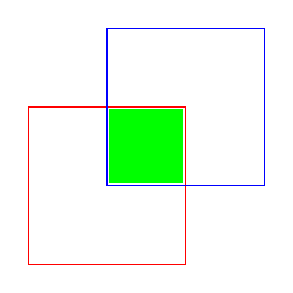
\begin{tikzpicture}
\draw [red] (0, 0) rectangle (2, 2);
\draw [blue] (1.0, 1.0) rectangle (3.0, 3.0);
\begin{scope}
	\fill[green] (1.03, 1.03) rectangle (1.97, 1.97);
\end{scope}
\end{tikzpicture}

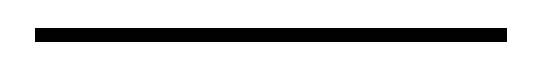
\begin{tikzpicture}
    \draw[line width=5pt,fill=black] (0,2) -- (6,2);
\end{tikzpicture}\vspace{0.2cm}%

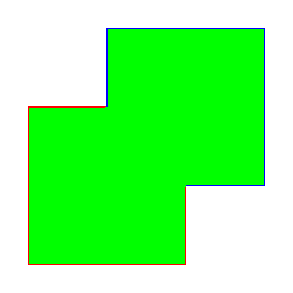
\begin{tikzpicture}
    \filldraw [draw=red,fill=green] (0, 0) rectangle (2, 2);
    \filldraw [draw=blue,fill=green] (1.0, 1.0) rectangle (3.0, 3.0);
    %\begin{scope}
			\fill[green] (0.98, 0.98) rectangle (2.0, 2.0);
		%\end{scope}
\end{tikzpicture}
\end{center}

% This is an example of how you would use tgrind to include an example
% of source code; it is commented out in this template since the code
% example file does not exist.  To use it, you need to remove the '%' on the
% beginning of the line, and insert your own information in the call.
%
%\tagrind[htbp]{code/pmn.s.tex}{Post Multiply Normalization}{opt:pmn}


\section{Data Acquisition}

Overview of caltech dataset
 \cite{dollar2011pedestrian}
which  includes   350,000  pedestrianbounding boxes (BB) labeled in 250,000 frames and remainsthe largest  such data  set to  date.

Challenges are there while just considering image data, 
the verities of image sources for example we can get photos that are taken by 
professionals, synthetic photos drawn by image generators and real life photos 
that we see and capture in our day to day life. So the results of these benchmarks and 
observation across these aforementioned classes of data set does not transfer to the other scenarios.

As already mentioned by \cite{walk2010new} Caltech data set is difficult for various reasons.
Many small pedestrians
realistic occlusion frequency
image quality is poor
includes blur
visible JPEG artifacts

\newpara
In our training data we had total number of BB for Person as a label=153234
sample data looks as below:
%frame,xmin,xmax,ymin,ymax,class_id
%set00_V000_1213.png,573,591,169,211,1
%set00_V000_1213.png,473,484,170,193,1
%set00_V000_166.png,406,418,164,187,1
%set00_V000_166.png,435,442,167,181,1
%set00_V000_166.png,233,241,120,134,1
%set00_V000_744.png,564,588,153,218,1
%set00_V000_744.png,565,587,173,206,1
%set00_V000_654.png,406,417,162,194,1
In 61439 unique images.
There are 72933 BB whose height is less than 50. As per \cite{walk2010new}, they considered 50-pixel-or-taller, unoccluded pedestrians, as they are not clear. Removing those BB where the height is less than 5o pixel, we are left with 80301 BBs in 37181 unique frames.
%df_with_height = df[(df['height'] >= 50) == True]
%df_with_width = df[(df['width'] <= 10) == True], gave us 519 such BBs where the width of the BB is less than or equals to 10 pixel. We also discarded such labels from our input training data set. We are finally left with 79831 BBs in 37081 unique frames.


%%% This is an example first chapter.  You should put chapter/appendix that you
%% write into a separate file, and add a line \include{yourfilename} to
%% main.tex, where `yourfilename.tex' is the name of the chapter/appendix file.
%% You can process specific files by typing their names in at the 
%% \files=
%% prompt when you run the file main.tex through LaTeX.
\chapter{Implementation and Results}
During the exploration and implementation of the Pedestrian intention prediction pipeline, SSD was chosen as the first block which acts as Pedestrian detector. In this chapter, how SSD was trained on large dataset, acquisition of data set and several aspect of Machine learning and Deep learning shall be discussed.

\section{Data Acqusition}
Challenges are there while just considering image data, the verities of image sources for example we can get photos that are taken by professionals, synthetic photos drawn by image generators and real life photos that we see and capture in our day to day life. So the results of these benchmarks and 
observation across these aforementioned classes of data set does not transfer to the other scenarios.
As recommended always for machine learning tasks, we should consider real data as close as possible to the environment where the designed system is expected to work. And luckily there exist some excellent data set in the public domain. I chose Caltech Data set \cite{dollar2009pedestrian}, which is one of the latest data set available in the public till today. 

\newpara
This data set contains highly annotated video, recorded from a moving vehicle in a normal trafic situation. It contains pedestrians vary largely in appearance, pose and scale. It also includes occlusion information. It contains close to 10 hours of recording at 30 fps with a video resolution 640 x 480. As seen and mentioned by the authors the overall image quality lower than that of same image resolution. The data set includes ~350,000  pedestrian bounding boxes (BB) labeled in 250,000frames and remains the largest such data set to  date. As already mentioned by \cite{walk2010new} Caltech data set is difficult for various reasons.

\begin{itemize}
	\setlength\itemsep{-1em}
	\item Many small pedestrians
	\item realistic occlusion frequency
	\item image quality is poor
	\item includes blur
	\item visible JPEG artifacts
\end{itemize}

\subsection{Data preparation}
After the video data got acquired, with help of a publicly available python project \cite{shuntasaito2015}, the original annotations in \textit{MATLAB} compatible \textit{vbb} format is converted to a JSON structure for easier consumption. The generated json file further processed and required data is extracted into a csv file using a python script located at \url{ https://github.com/Kalinga/ML/blob/master/ssd_keras_caltech/json_anno_csv_conversion.ipynb}. As mentioned by \cite{dollar2009pedestrian} the video set from 00-05 is expected for training purpose and 06-10 is for testing purpose.

In the Caltech data group of people are separately label as \textit{people}. With the intention, the ML model should learn individual person and identify persons rather than people, when there are several persons close by, i decided to remove \textit{people} class label from the training data set. And also the number of samples for \textit{people} and \textit{person} was disproportionately varying. This was another reason to exclude \textit{people }label from  the training. The frequency for the both classes are shown as below.

\begin{figure}[H]
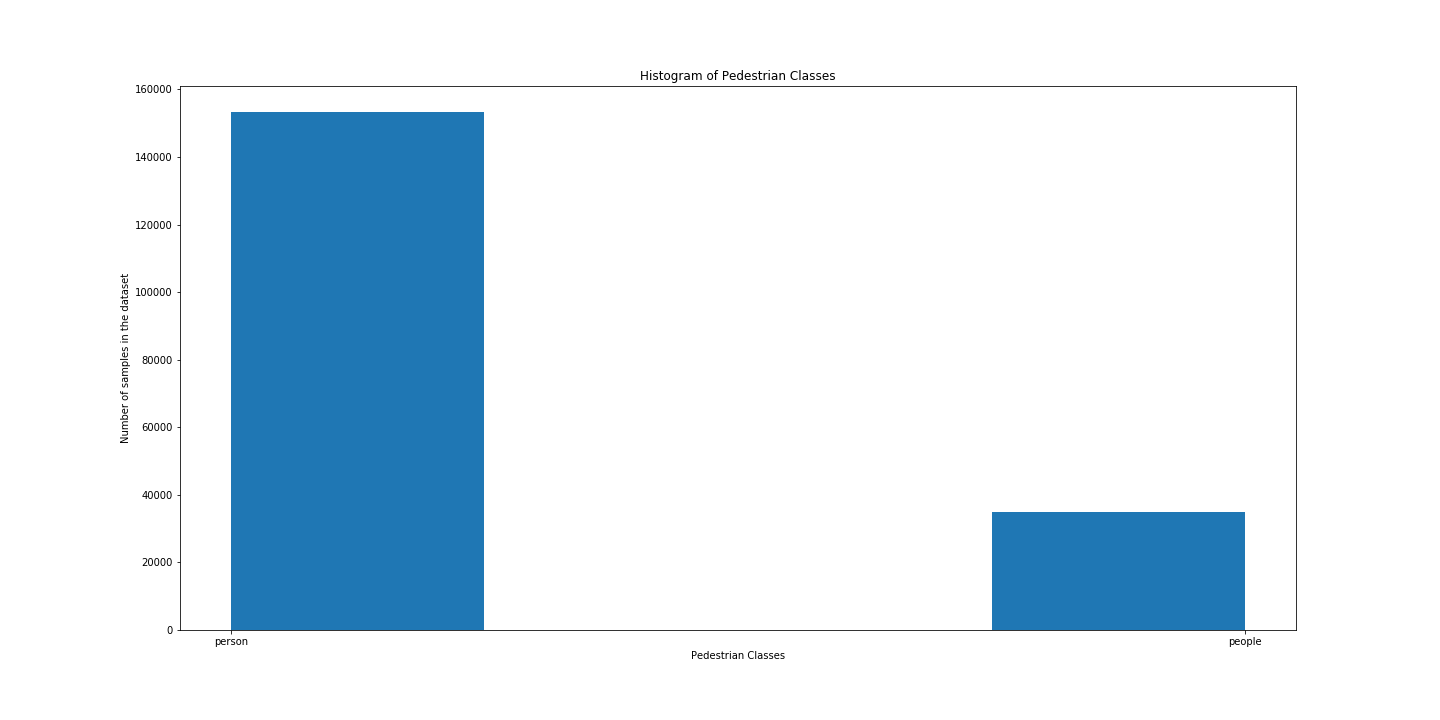
\includegraphics[scale=0.4]{classid_distribution1_2}
\begin{center}
\caption{Class 'person' and 'people' distribution}
\end{center}
\end{figure}

As per \cite{walk2010new}, unoccluded pedestrians with 50-pixel-or-taller are considered , as they are not clear. For simplicity purpose below data are discarded from the training set.
\begin{itemize}
	\item Class label with \textit{people}, \textit{person-fa}, \textit{person?}
	\item occluded \textit{person} label
	\item images below 50 pixel in height
	\item images below 5 pixel in width
\end{itemize}

After the above mentioned clean up, our training data contains total 48194 number of BB with person as a label in 26902 unique frames and sample data looks as below:
\begin{center}
\texttt{  \\
frame,xmin,xmax,ymin,ymax,class\textunderscore id \\
set00\textunderscore V000\textunderscore 1213.png,573,591,169,211,1 \\
set00\textunderscore V000\textunderscore 1213.png,473,484,170,193,1 \\
set00\textunderscore V000\textunderscore 166.png,406,418,164,187,1 \\
set00\textunderscore V000\textunderscore 166.png,435,442,167,181,1 \\
set00\textunderscore V000\textunderscore 166.png,233,241,120,134,1 \\
set00\textunderscore V000\textunderscore 744.png,564,588,153,218,1 \\
set00\textunderscore V000\textunderscore 744.png,565,587,173,206,1 \\
set00\textunderscore V000\textunderscore 654.png,406,417,162,194,1 \\
}
\end{center}

During the training an NVIDIA GeForce GTX 1080 GPU with 8GB of video memory was used, while using a validation data size equals to standard 10\% of training data, the training time was equals to unusable, as training of a single epoch was taking nearly ~30-40 hours. The experiment was run on a shared Linux server hosted within the University Network and the computing resource was shared with other students. Keeping this in view, i decided to reduce the size of the validation data set size to great extent and get an approximate impression about the model's training efficiency. Below table show the training and validation data partition.

\begin {table}[H]
\begin{center}
 \begin{tabular}{||c c c||}
 \hline
 Data Set & Bounding Box & Frames\\ [0.8ex] 
 \hline\hline
 Training & 47194 & 26280 \\
 \hline
 Validation & 1000 & 622 \\
 \hline
 Total & 48194 & 26902 \\
 \hline
\end{tabular}
\caption{Training and Validation sample numbers}
\end{center}
\end {table}

\cite{dollar2009pedestrian} defines pedestrians with 80 pixels or taller as in the near scale and 30 pixel or less
are in the far scale and rest in the medium scale. Most pedestrians are observed in medium scale. A person with 1.8m tall is 1.5s away from the vehicle for the mentioned set up and speed of 55km\/h. \cite{dollar2011pedestrian} shows that average aspect ratio \textit{$w \approx 0.41h$}. After above mentioned cleaning steps, a re calculation for the aspect ration distribution shows, it does not vary much from the original distribution, as shown below.

\begin{figure}[H]
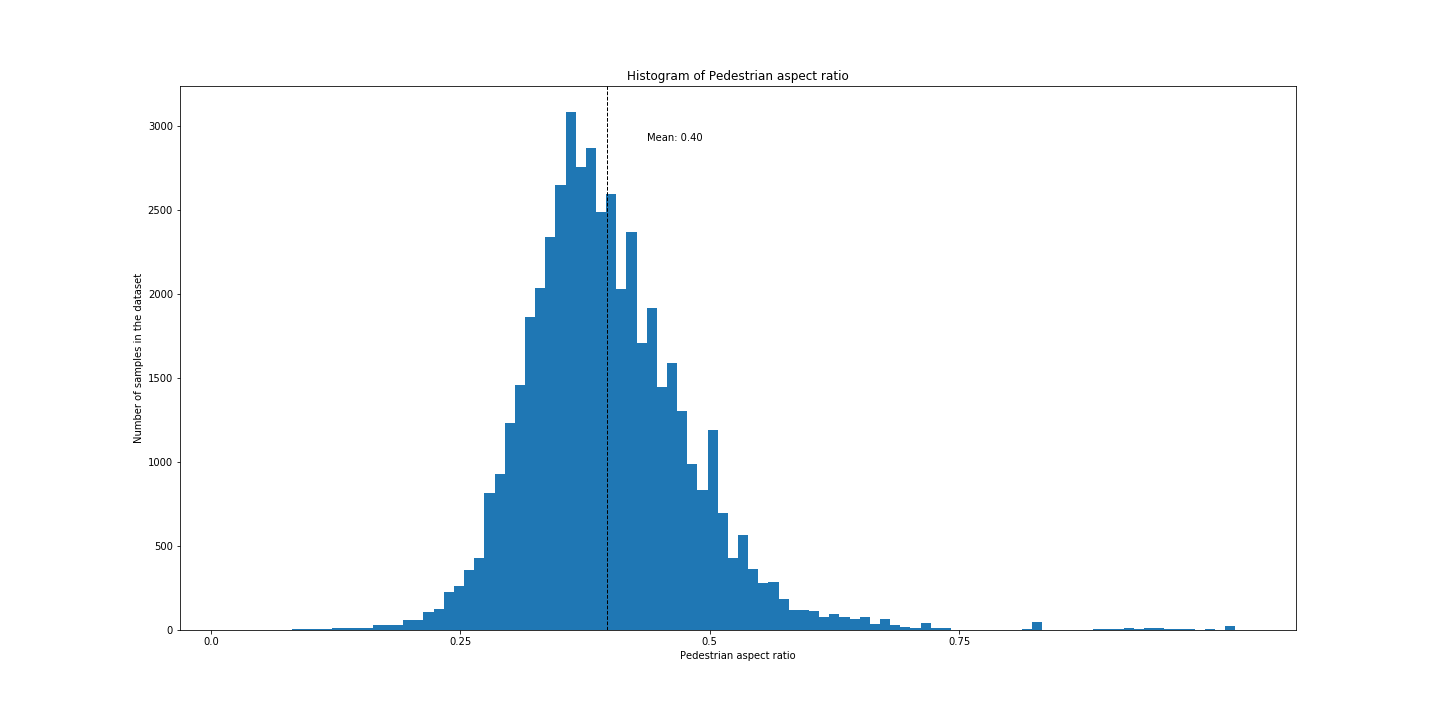
\includegraphics[scale=0.4]{aspect_ratio_distribution}
\begin{center}
\caption{Pedestrian aspect ratio distribution}
\end{center}
\end{figure}

\section{Training }
As SSD has predictors at multiple level, before the model training step, a pre-processing step is required where proposed BBs are generated and compared with the ground truth and depending on IoU threshold, certain prior BBs are considered and encoded for the training purpose. There are several parameters play a role in generating bounding boxes and some of critical parameters used are given below.

\subsection{Framework parameters}

\begin {table}[H]
\begin{center}
 \begin{tabular}{||c c||} 
 \hline
 Param. Name & Value\\ [0.8ex] 
 \hline\hline
 img\textunderscore  height & 480 \\ 
 \hline
 img\textunderscore  width & 640 \\
 \hline
 img\textunderscore  channels & 3 \\
 \hline
 n\textunderscore  classes & 1 \\
 \hline
 scales & $[0.08, 0.16, 0.32, 0.64, 0.96]$ \\
 \hline
\end{tabular}
\caption{SSD framework parameters}
\end{center}
\end{table}

\subsection{Model parameters}
\textbf{Model Architecture:}
SSD model consists of convolutional feature layers and some convolutional predictor layers that take input from different feature layers, making the model fully convolutional. In the presented model, 7 convolutional layers and 4 predictors layers are used. These 4 convolutional predictors layers take input from layers 4, 5, 6, and 7 respectively. convnet with was used for modeling using keras \footnote{Keras is a high-level neural networks API, written in Python and capable of running on top of TensorFlow, CNTK, or Theano.}. The model is created and initialised with Keras API Sequential (). 

\subsection{Hyper Parameters}

\subsection{ Validation: Graphs and results}

\begin{figure}[H]
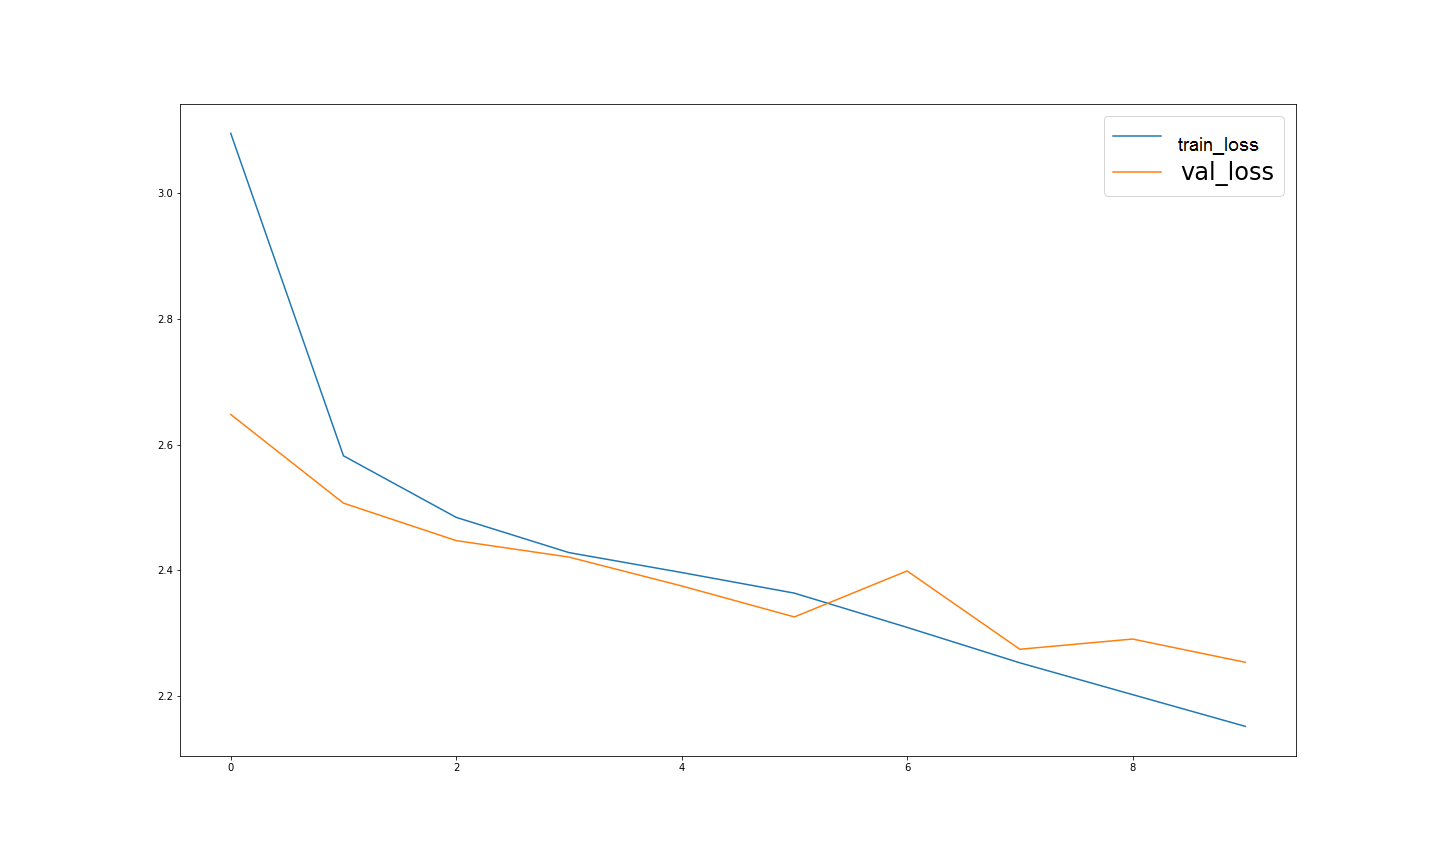
\includegraphics[scale=0.4]{conf0_loss-val_loss_0_10epochs}
\begin{center}
\caption{Training and Validation error at 10 epochs}
\end{center}
\end{figure}
As the training error has not converged after 10 epochs it was decided to training for another 10 epoch and the graph as follows. After training for 10 epochs the training error gradually reduces and the validation error revolves around training error as shown in the below graph. As the training of single epoch takes significant time the statistics were taken with small epochs.

\begin{figure}[H]
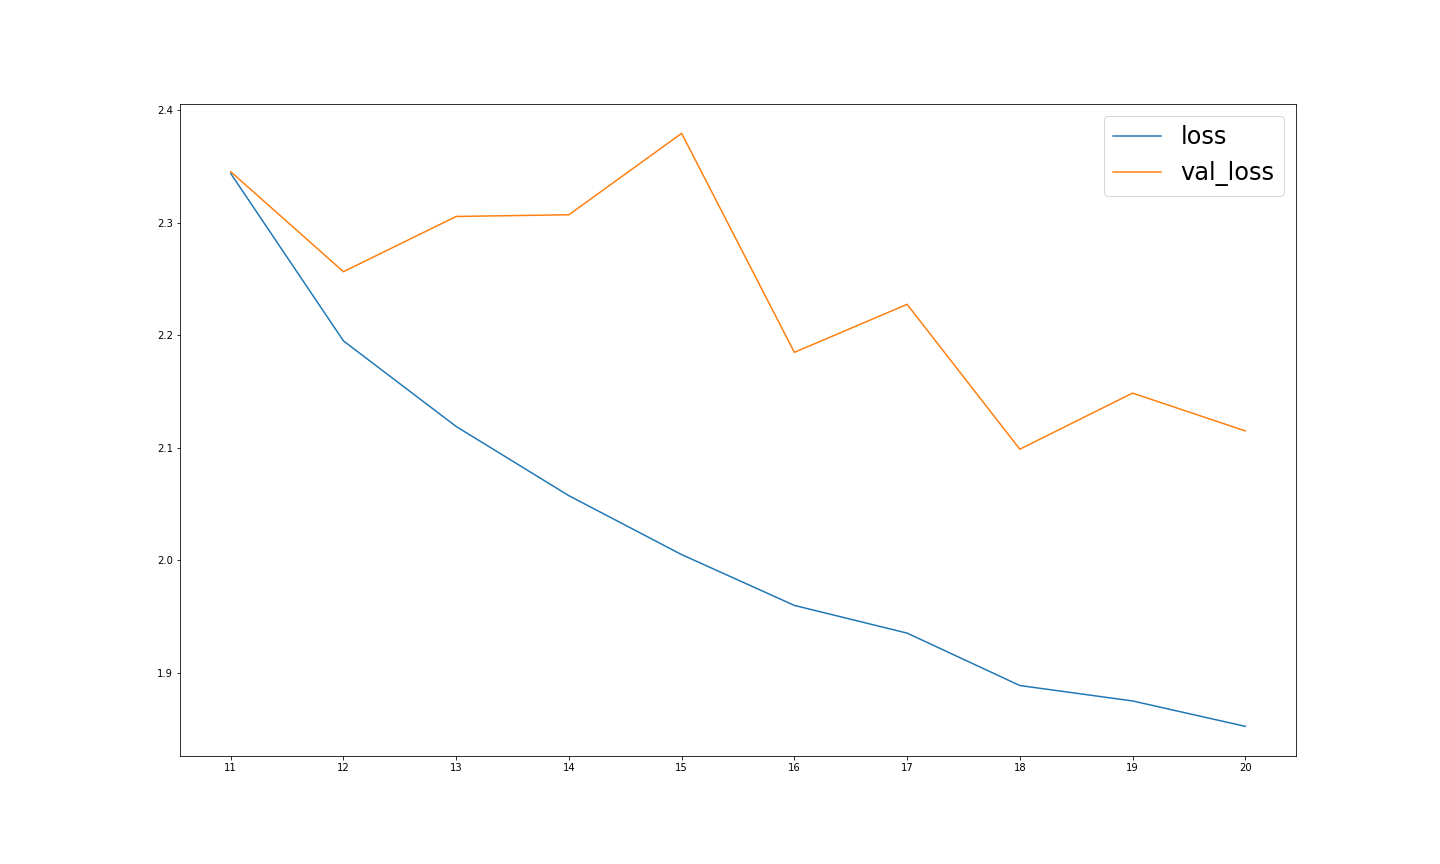
\includegraphics[scale=0.4]{conf0_loss-val_loss_10_20epochs}
\begin{center}
\caption{Training and Validation error at 20 epochs}
\end{center}
\end{figure}

\newpara
Looking at the graph which depicts training loss and validation loss drawn with several epochs, we could see training error gradually reduces with increase in the number of epochs, simultaneously we see validation loss also exhibiting same pattern and slowly decreasing with number of epochs. This trend of decrease in validation error with increase in training is a good indication of learning. The model could have trained for some more epochs until it converges, however due to long training time, it was not possible to do so, instead training with different configuration was done to see the behavior with other configuration.

\section{Testing} 
For the testing of the generated model below steps were followed to prepare the test data and conduct the experiment.
\begin{enumerate}
	\item video set 06 - 10 was selected as test data and bounding box, label are extracted into labels\textunderscore test\textunderscore full.csv which contains total 154436 records
	\item Rows with occluded and other classes except person were removed and remaining number of records were 73218, which consists of 42910 unique images 
	\item records with less than 50 pixel for height or 5 pixel for width were discarded and data set left with 29620 records
	\item From the above data 1000 records were randomly chosen for test purpose which consists of 902 unique images
\end{enumerate}

\newpara
While using SSD7, it was observed that, the algorithm is very sensitive to the list of aspect ratios for the anchor boxes. To begin with, the values for aspect\textunderscore ratios = $[0.5, 1.0, 2.0]$ were used and that lead to very poor result in the evaluation phase. Subsequently the model was trained with several different configuration and results are noted as below.

for aspect\textunderscore ratios = $[0.1, 0.2, 0.33, 0.413, 0.418, 0.5, 0.6, 0.7, 0.8, 1.0]$
\begin{table}[H]
\begin{center}
 \begin{tabular}{||c c c||} 
 \hline
 No. epoch & mAP & fps\\ [0.8ex] 
 \hline\hline
 10 & 0.661 & 10.22\\ 
 \hline
 20  & 0.635 & 9.73 \\
\hline
\end{tabular}
\caption{Average Precision and fps with number of epochs}
\end{center}
\end{table}
From the above result, it can be observed that training the data for more epochs actually not resulting a better model as both mAP and fps is lowered for the model trained with 20 epochs, this could be sign of \textit{over-fitting.}


conf1
0.2, 0.33, 0.413, 0.418, 0.5, 0.6, 0.7, 0.8, 1.0
0.4376
fps 73.14

conf 2
epoch 5
0.1, 0.2, 0.33, 0.413, 0.418, 0.5, 0.6, 0.7, 0.8
fps: 75.58 
mAP:0.471

conf 3 
0.1, 0.2, 0.33, 0.413, 0.418, 0.5, 0.6, 0.7, 0.8, 1.0





With the increase in number of values in the list of aspect ratio, the number of predictor boxes increases. Increase in number of predictor boxes increases both training time as well as prediction time.

\section{JAAD Dataset}

JAAD \cite{rasouli2017agreeing} is a publicly available large scale data set that includes data for pedestrian detection with behavioral and contextual information. It contains 346 video clips of pedestrian data that includes occlusion label, temporal correlation, behavioral aspect, contextual information weather related data. Rasouli et al. provided a supporting GitHub code for easier interaction with JAAD data. The videos can be downloaded by running the script \colorbox{lightgray}{download\textunderscore clips.sh}. The video clips are downloaded into JAAD\textunderscore clips and the clips are named as below.\\
\colorbox{lightgray} {JAAD\textunderscore clips/video\textunderscore  0001.mp4} \\
\colorbox{lightgray} {JAAD\textunderscore clips/video\textunderscore  0002.mp4}

Using \colorbox{lightgray}{split\textunderscore clips\textunderscore to\textunderscore .sh} the frames are extracted to corresponding video id directory with in a floder called \textit{images} \\
\begin{center}
\colorbox{lightgray} {images/video\textunderscore  0001/0000.png} \\
\colorbox{lightgray} {images/video\textunderscore  0001/0001.png} \\
\colorbox{lightgray} {....}
\end{center}

In JAAD annotations are divided into 5 groups:
\begin{itemize}
	\item Annotations: Information about pedestrian bounding box, occlusion information, activities. These annotations are one per frame per label.
	\item Attribute: Contains information regarding pedestrian’s crossing points, crossing characteristics. These annotations are one per pedestrian.
	\item Appearance: Information regarding pedestrian pose, clothing, objects they carry. These information are one per frame per pedestrian.
	\item Traffic: Includes information about traffic signs, traffic light for each frame.
	\item Vehicle: Per frame vehicle speed information e.g moving fast, speeding up.
\end{itemize}


The early work includes prediction of road users behavior by employing dynamic factors e.g trajectory prediction, velocity prediction or predicting final goal of the pedestrian. Recently behavioral aspect such as awareness by estimating head orientation along with other contextual information such as sign, weather condition, visibility and individual characteristics of the pedestrian such as things he carry, age and sex, size of the group he is associated with influence crossing behavior.

TODO:  pedestrian to identify the pedestrians with behavioral tags (i.e. the ones demonstrating the intention of crossing or located close to the curb). 
Occlusion information is provided in the form of tags for
each bounding box: partial occlusion (between 25\% and 75\%
visible) and full occlusion (less than 25\% visible).
 654 unique pedestrian samples (out of 2.2k samples) with behavioral tags in the
dataset. 
The
pedestrians\' actions are categorized into 3 groups: Precondition- this refers to the state of the pedestrian prior to crossing and can be either standing, moving slow or fast. Attention- the way the pedestrian becomes aware of the approaching vehicle. These actions, depending on their duration, are looking ( > 1s) or glancing ($\leq$ 1s). Response- this
includes the behaviors that pedestrians exhibit in response
to the action of the approaching vehicle, namely, stop, clear path, slow down, speed up, hand gesture and nod.

\subsection{LSTM results}
With the below information from JAAD team, i decided to model the data using videos 71-346.
Video data from 317-346, 30 videos data is separated and was kept for model testing purpose.
Remaining 246 (71-316) video data was used for training and validation purpose.
During the training and validation, from total available for training 84372 bounding box information, 20000 bbs used for validation which is around 23.7\% of totaol training data.

Test RMSE represents testing the model with frames extracted from one video from the test set.
conf1: model with epochs = 1000, MinMaxScaler(feature\textunderscore range=(0, 1)), 
number of sequence as observation = 3
loss: 0.0045 - val\textunderscore loss: 0.0047 
Test RMSE: 2.363
Validation: Using one pedestrian bounding boxes with 205 frames.
% git commit 789d6e6

conf2: 
model with epochs = 200, early stopping after epoch 33
number of sequence as observation = 15
loss: 0.0087 - val\textunderscore loss: 0.0089
Test RMSE: 4.749
%9c88a25

conf3:
model with epochs = 200, early stopping after epoch 88
loss-0.0062 val\textunderscore loss-0.0070.h5
model with epochs = 200
number of sequence as observation = 30
Test RMSE: 4.625


%model.add(LSTM(50, input\textunderscoreshape=(train\textunderscoreX.shape[1], train\textunderscoreX.shape[2])))
vid = "video\textunderscore0318"
total \#prediction: 179
total time: 2.909117
avg prediction speed: 0.016252
total positive: 113
accuracy: 0.631285

%model.add(LSTM(30, input\textunderscoreshape=(train\textunderscoreX.shape[1], train\textunderscoreX.shape[2])))
total \#prediction: 179
total time: 3.122547
avg prediction speed: 0.017444
total positive: 57
accuracy: 0.318436

total \#prediction: 180
total time: 3.063958
avg prediction speed: 0.017022
total positive: 57
accuracy: 0.316667

%ls cm-pm | wc -l 185      *2  370
%ls cm-ps | wc -l 142 145  *3  335
%ls cms-pm | wc -l 245 245 *2  490
%ls cms-ps | wc -l 37 40   *12 480
%ls cs-pm| wc -l 173 175   *2  350
%ls cs-ps | wc -l 15 15    *30 450

%Train on 342135 samples, validate on 85534 samples
%Epoch 1/300
%Started at 17th sept 15:45 
Annotations for the video can be extracted as below
anno = imdb.\textunderscore get\textunderscore annotations(vid), this results in a dictionary which contains below keys ['height', 'ped\textunderscore annotations', 'num\textunderscore frames', 'width']

TODO
\newpara Weakly supervised learning!
Sigmoid cross entropy vs  softmax
batch normalization


\subsection{Problem}
MinMax scalar at a global scale introduce the error

%%% This is an example first chapter.  You should put chapter/appendix that you
%% write into a separate file, and add a line \include{yourfilename} to
%% main.tex, where `yourfilename.tex' is the name of the chapter/appendix file.
%% You can process specific files by typing their names in at the 
%% \files=
%% prompt when you run the file main.tex through LaTeX.
\chapter{Simulation, Results and Discussion}
During the exploration and implementation of the Pedestrian intention prediction pipeline, SSD was chosen as the first block which acts as Pedestrian detector. In this chapter, how SSD was trained on large dataset, acquisition of data set and several aspect of Machine learning and Deep learning shall be discussed.

\section{Data Acquisition}
Challenges are there while just considering image data, the verities of image sources for example we can get photos that are taken by professionals, synthetic photos drawn by image generators and real life photos that we see and capture in our day to day life. So the results of these benchmarks and 
observation across these aforementioned classes of data set does not transfer to the other scenarios.
As recommended always for machine learning tasks, we should consider real data as close as possible to the environment where the designed system is expected to work. And luckily there exist some excellent data set in the public domain. I chose Caltech Data set \cite{dollar2009pedestrian}, which is one of the latest data set available in the public till today. 

\newpara
This data set contains highly annotated video, recorded from a moving vehicle in a normal trafic situation. It contains pedestrians vary largely in appearance, pose and scale. It also includes occlusion information. It contains close to 10 hours of recording at 30 fps with a video resolution 640 x 480. As seen and mentioned by the authors the overall image quality lower than that of same image resolution. The data set includes ~350,000  pedestrian bounding boxes (BB) labeled in 250,000frames and remains the largest such data set to  date. As already mentioned by \cite{walk2010new} Caltech data set is difficult for various reasons.

\begin{itemize}
	\setlength\itemsep{-1em}
	\item Many small pedestrians
	\item realistic occlusion frequency
	\item image quality is poor
	\item includes blur
	\item visible JPEG artifacts
\end{itemize}

\subsection{Data preparation}
After the video data got acquired, with help of a publicly available python project \cite{shuntasaito2015}, the original annotations in \textit{MATLAB} compatible \textit{vbb} format is converted to a JSON structure for easier consumption. The generated json file further processed and required data is extracted into a csv file using a python script located at \url{ https://github.com/Kalinga/ML/blob/master/ssd_keras_caltech/json_anno_csv_conversion.ipynb}. As mentioned by \cite{dollar2009pedestrian} the video set from 00-05 is expected for training purpose and 06-10 is for testing purpose.

In the Caltech data group of people are separately label as \textit{people}. With the intention, the ML model should learn individual person and identify persons rather than people, when there are several persons close by, i decided to remove \textit{people} class label from the training data set. And also the number of samples for \textit{people} and \textit{person} was disproportionately varying. This was another reason to exclude \textit{people }label from  the training. The frequency for the both classes are shown as below.

\begin{figure}[H]
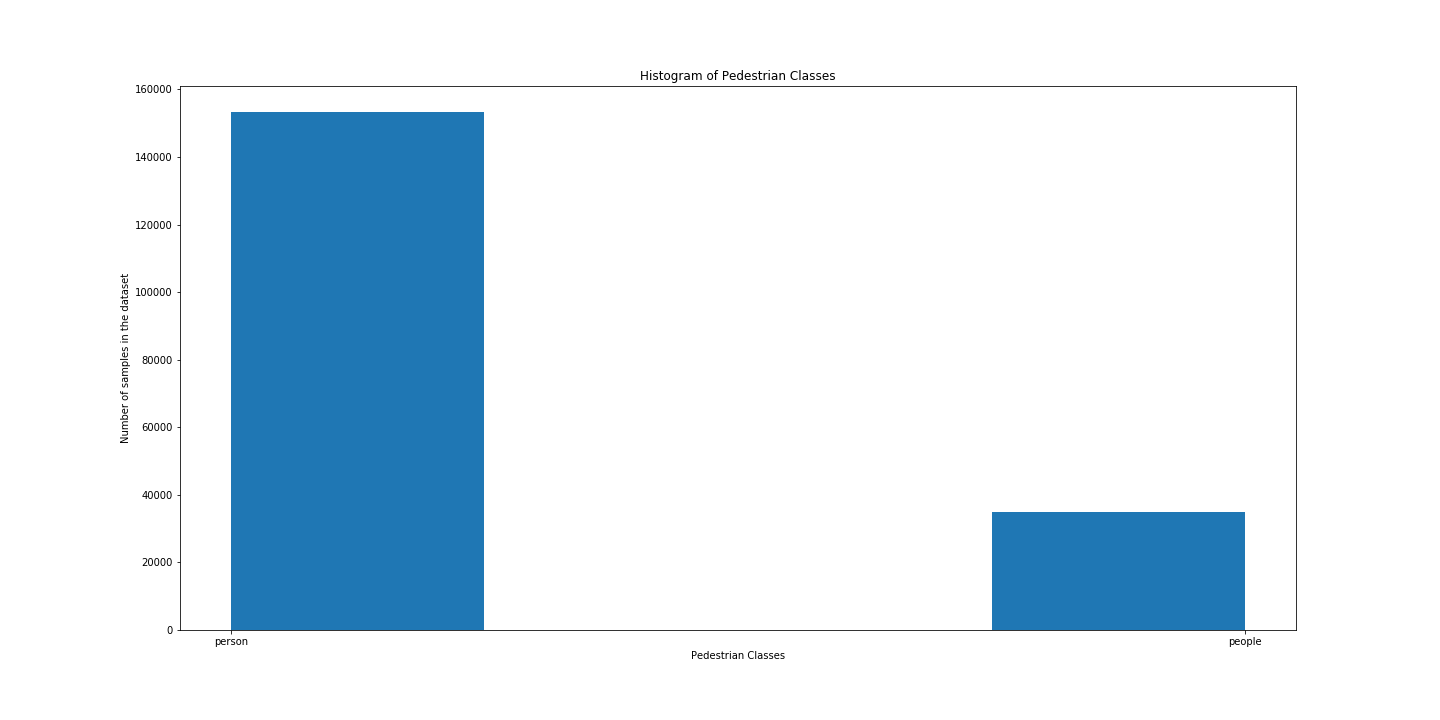
\includegraphics[scale=0.4]{classid_distribution1_2}
\begin{center}
\caption{Class 'person' and 'people' distribution}
\end{center}
\end{figure}

As per \cite{walk2010new}, unoccluded pedestrians with 50-pixel-or-taller are considered , as they are not clear. For simplicity purpose below data are discarded from the training set.
\begin{itemize}
	\item Class label with \textit{people}, \textit{person-fa}, \textit{person?}
	\item occluded \textit{person} label
	\item images below 50 pixel in height
	\item images below 5 pixel in width
\end{itemize}

After the above mentioned clean up, our training data contains total 48194 number of BB with person as a label in 26902 unique frames and sample data looks as below:
\begin{center}
\texttt{  \\
frame,xmin,xmax,ymin,ymax,class\textunderscore id \\
set00\textunderscore V000\textunderscore 1213.png,573,591,169,211,1 \\
set00\textunderscore V000\textunderscore 1213.png,473,484,170,193,1 \\
set00\textunderscore V000\textunderscore 166.png,406,418,164,187,1 \\
set00\textunderscore V000\textunderscore 166.png,435,442,167,181,1 \\
set00\textunderscore V000\textunderscore 166.png,233,241,120,134,1 \\
set00\textunderscore V000\textunderscore 744.png,564,588,153,218,1 \\
set00\textunderscore V000\textunderscore 744.png,565,587,173,206,1 \\
set00\textunderscore V000\textunderscore 654.png,406,417,162,194,1 \\
}
\end{center}

During the training an NVIDIA GeForce GTX 1080 GPU with 8GB of video memory was used, while using a validation data size equals to standard 10\% of training data, the training time was equals to unusable, as training of a single epoch was taking nearly ~30-40 hours. The experiment was run on a shared Linux server hosted within the University Network and the computing resource was shared with other students. Keeping this in view, i decided to reduce the size of the validation data set size to great extent and get an approximate impression about the model's training efficiency. Below table show the training and validation data partition.

\begin {table}[H]
\begin{center}
 \begin{tabular}{||c c c||}
 \hline
 Data Set & Bounding Box & Frames\\ [0.8ex] 
 \hline\hline
 Training & 47194 & 26280 \\
 \hline
 Validation & 1000 & 622 \\
 \hline
 Total & 48194 & 26902 \\
 \hline
\end{tabular}
\caption{Training and Validation sample numbers}
\end{center}
\end {table}

\cite{dollar2009pedestrian} defines pedestrians with 80 pixels or taller as in the near scale and 30 pixel or less
are in the far scale and rest in the medium scale. Most pedestrians are observed in medium scale. A person with 1.8m tall is 1.5s away from the vehicle for the mentioned set up and speed of 55km\/h. \cite{dollar2011pedestrian} shows that average aspect ratio \textit{$w \approx 0.41h$}. After above mentioned cleaning steps, a re calculation for the aspect ration distribution shows, it does not vary much from the original distribution, as shown below.

\begin{figure}[H]
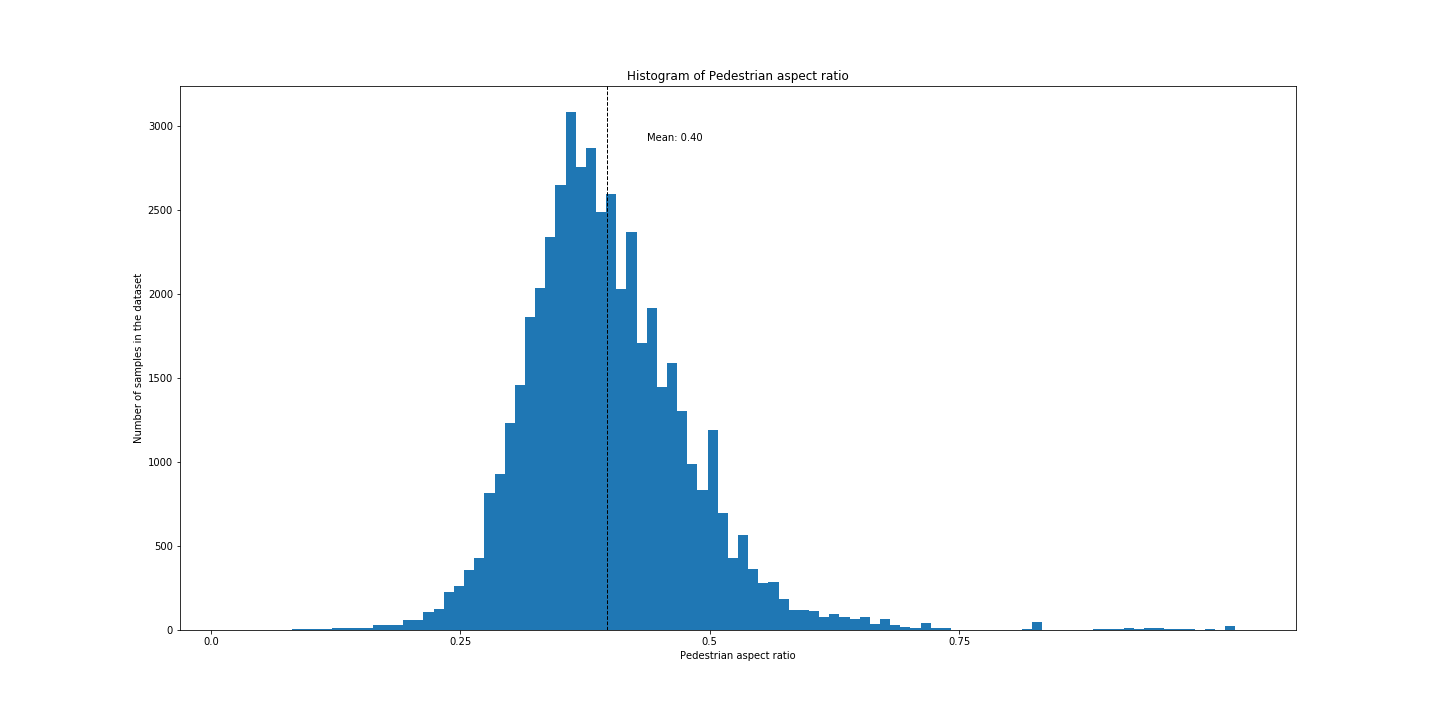
\includegraphics[scale=0.4]{aspect_ratio_distribution}
\begin{center}
\caption{Pedestrian aspect ratio distribution}
\end{center}
\end{figure}

\section{Training }
As SSD has predictors at multiple level, before the model training step, a pre-processing step is required where proposed BBs are generated and compared with the ground truth and depending on IoU threshold, certain prior BBs are considered and encoded for the training purpose. There are several parameters play a role in generating bounding boxes and some of critical parameters used are given below.

\subsection{Framework parameters}

\begin {table}[H]
\begin{center}
 \begin{tabular}{||c c||} 
 \hline
 Param. Name & Value\\ [0.8ex] 
 \hline\hline
 img\textunderscore  height & 480 \\ 
 \hline
 img\textunderscore  width & 640 \\
 \hline
 img\textunderscore  channels & 3 \\
 \hline
 n\textunderscore  classes & 1 \\
 \hline
 scales & $[0.08, 0.16, 0.32, 0.64, 0.96]$ \\
 \hline
\end{tabular}
\caption{SSD framework parameters}
\end{center}
\end{table}

\subsection{Model parameters}
\textbf{Model Architecture:}
SSD model consists of convolutional feature layers and some convolutional predictor layers that take input from different feature layers, making the model fully convolutional. In the presented model, 7 convolutional layers and 4 predictors layers are used. These 4 convolutional predictors layers take input from layers 4, 5, 6, and 7 respectively. convnet with was used for modeling using keras \footnote{Keras is a high-level neural networks API, written in Python and capable of running on top of TensorFlow, CNTK, or Theano.}. The model is created and initialised with Keras API Sequential (). 

\subsection{Hyper Parameters}

\subsection{ Validation: Graphs and results}

\begin{figure}[H]
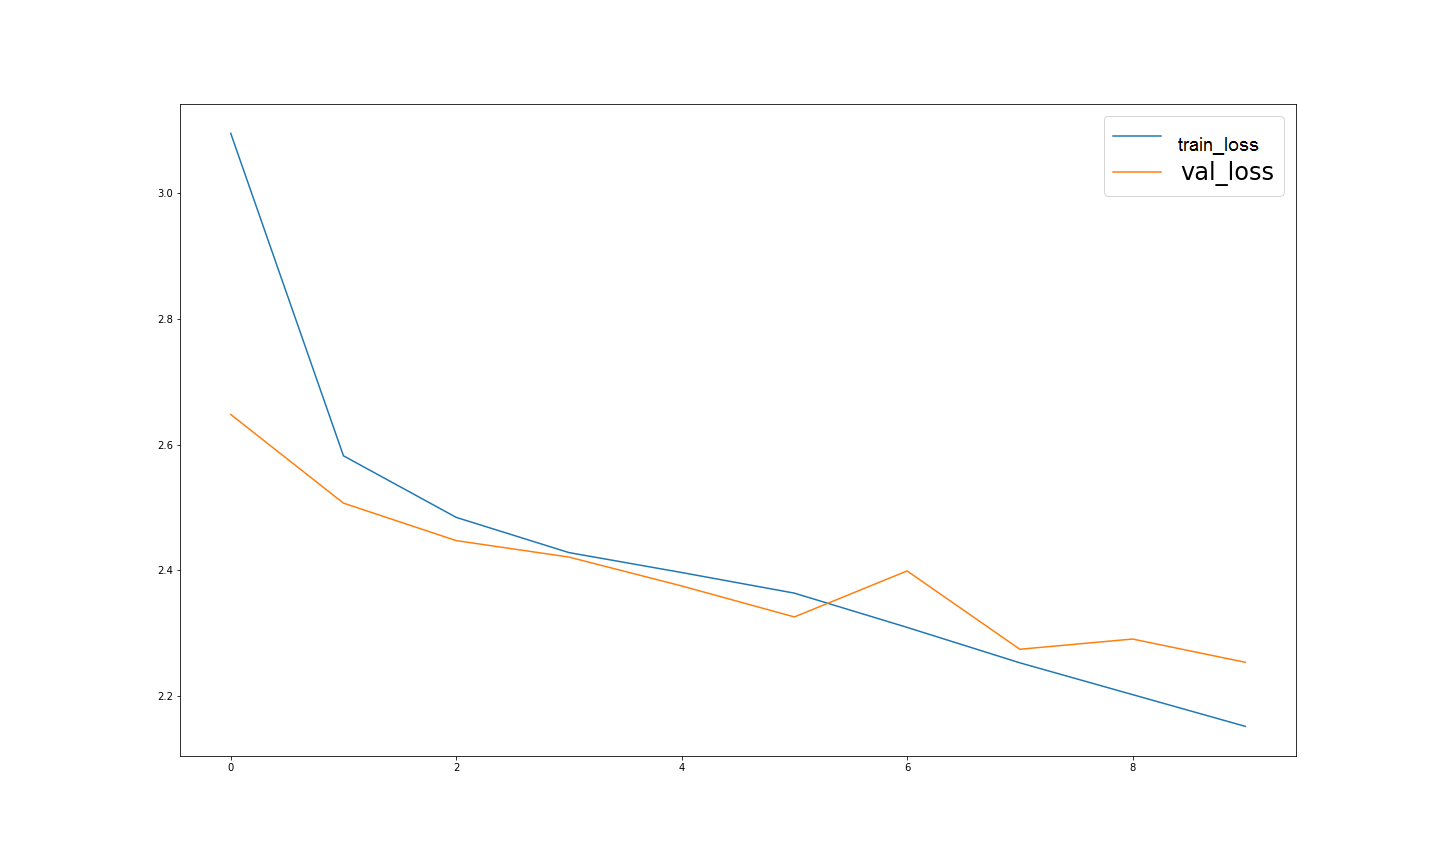
\includegraphics[scale=0.4]{conf0_loss-val_loss_0_10epochs}
\begin{center}
\caption{Training and Validation error at 10 epochs}
\end{center}
\end{figure}
As the training error has not converged after 10 epochs it was decided to training for another 10 epoch and the graph as follows. After training for 10 epochs the training error gradually reduces and the validation error revolves around training error as shown in the below graph. As the training of single epoch takes significant time the statistics were taken with small epochs.

\begin{figure}[H]
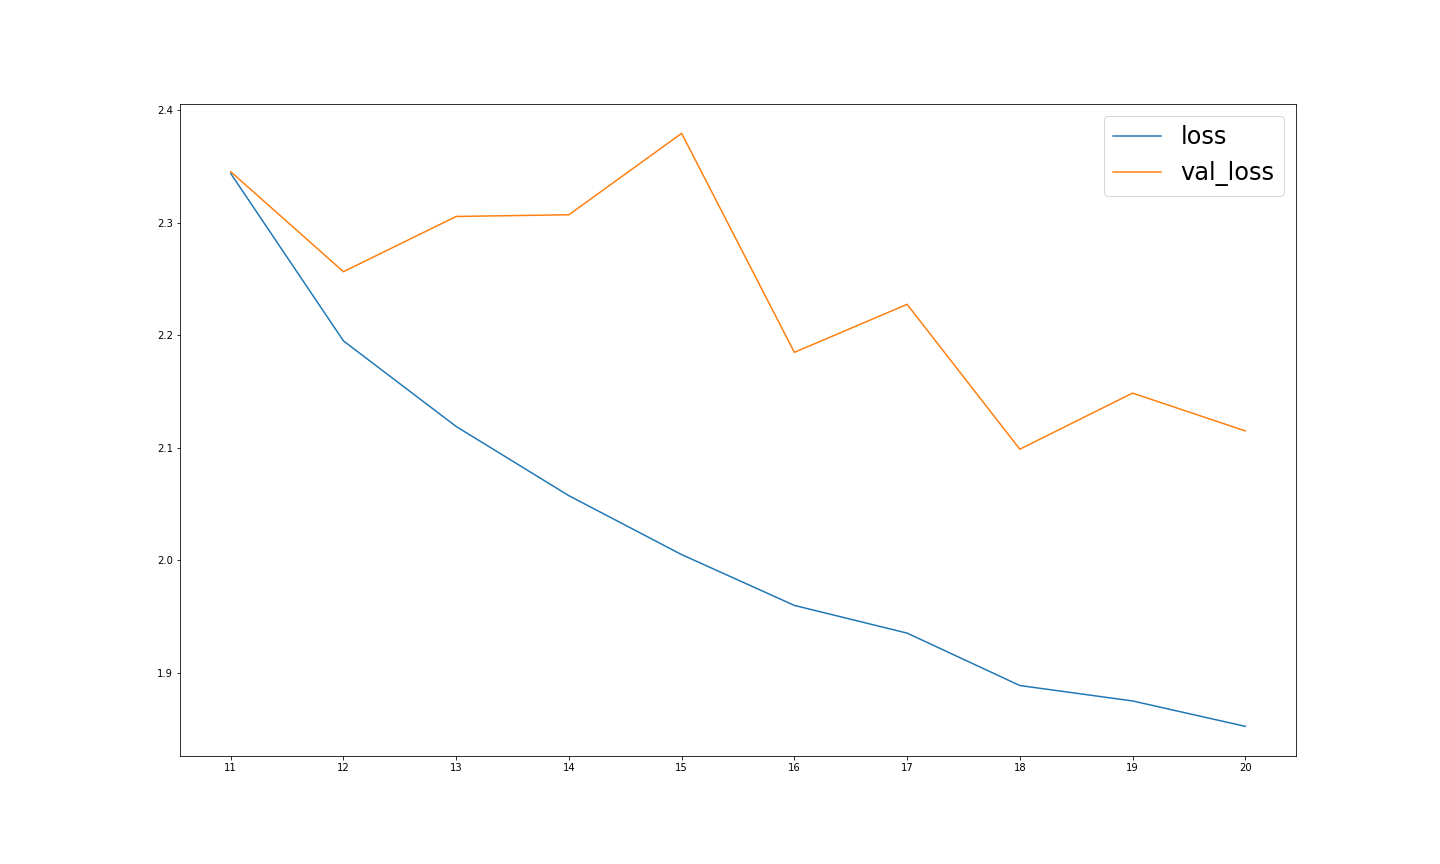
\includegraphics[scale=0.4]{conf0_loss-val_loss_10_20epochs}
\begin{center}
\caption{Training and Validation error at 20 epochs}
\end{center}
\end{figure}

\newpara
Looking at the graph which depicts training loss and validation loss drawn with several epochs, we could see training error gradually reduces with increase in the number of epochs, simultaneously we see validation loss also exhibiting same pattern and slowly decreasing with number of epochs. This trend of decrease in validation error with increase in training is a good indication of learning. The model could have trained for some more epochs until it converges, however due to long training time, it was not possible to do so, instead training with different configuration was done to see the behavior with other configuration.

\section{Testing} 
For the testing of the generated model below steps were followed to prepare the test data and conduct the experiment.
\begin{enumerate}
	\item video set 06 - 10 was selected as test data and bounding box, label are extracted into labels\textunderscore test\textunderscore full.csv which contains total 154436 records
	\item Rows with occluded and other classes except person were removed and remaining number of records were 73218, which consists of 42910 unique images 
	\item records with less than 50 pixel for height or 5 pixel for width were discarded and data set left with 29620 records
	\item From the above data 1000 records were randomly chosen for test purpose which consists of 902 unique images
\end{enumerate}

\newpara
While using SSD7, it was observed that, the algorithm is very sensitive to the list of aspect ratios for the anchor boxes. To begin with, the values for aspect\textunderscore ratios = $[0.5, 1.0, 2.0]$ were used and that lead to very poor result in the evaluation phase. Subsequently the model was trained with several different configuration and results are noted as below.

for aspect\textunderscore ratios = $[0.1, 0.2, 0.33, 0.413, 0.418, 0.5, 0.6, 0.7, 0.8, 1.0]$
\begin{table}[H]
\begin{center}
 \begin{tabular}{||c c c||} 
 \hline
 No. epoch & mAP & fps\\ [0.8ex] 
 \hline\hline
 10 & 0.661 & 10.22\\ 
 \hline
 20  & 0.635 & 9.73 \\
\hline
\end{tabular}
\caption{Average Precision and fps with number of epochs}
\end{center}
\end{table}
From the above result, it can be observed that training the data for more epochs actually not resulting a better model as both mAP and fps is lowered for the model trained with 20 epochs, this could be sign of \textit{over-fitting.}


conf1
0.2, 0.33, 0.413, 0.418, 0.5, 0.6, 0.7, 0.8, 1.0
0.4376
fps 73.14

conf 2
epoch 5
0.1, 0.2, 0.33, 0.413, 0.418, 0.5, 0.6, 0.7, 0.8
fps: 75.58 
mAP:0.471

conf 3 
0.1, 0.2, 0.33, 0.413, 0.418, 0.5, 0.6, 0.7, 0.8, 1.0





With the increase in number of values in the list of aspect ratio, the number of predictor boxes increases. Increase in number of predictor boxes increases both training time as well as prediction time.

\section{JAAD Dataset}

JAAD \cite{rasouli2017agreeing} is a publicly available large scale data set that includes data for pedestrian detection with behavioral and contextual information. It contains 346 video clips of pedestrian data that includes occlusion label, temporal correlation, behavioral aspect, contextual information weather related data. Rasouli et al. provided a supporting GitHub code for easier interaction with JAAD data. The videos can be downloaded by running the script \colorbox{lightgray}{download\textunderscore clips.sh}. The video clips are downloaded into JAAD\textunderscore clips and the clips are named as below.\\
\colorbox{lightgray} {JAAD\textunderscore clips/video\textunderscore  0001.mp4} \\
\colorbox{lightgray} {JAAD\textunderscore clips/video\textunderscore  0002.mp4}

Using \colorbox{lightgray}{split\textunderscore clips\textunderscore to\textunderscore .sh} the frames are extracted to corresponding video id directory with in a floder called \textit{images} \\
\begin{center}
\colorbox{lightgray} {images/video\textunderscore  0001/0000.png} \\
\colorbox{lightgray} {images/video\textunderscore  0001/0001.png} \\
\colorbox{lightgray} {....}
\end{center}

In JAAD annotations are divided into 5 groups:
\begin{itemize}
	\item Annotations: Information about pedestrian bounding box, occlusion information, activities. These annotations are one per frame per label.
	\item Attribute: Contains information regarding pedestrian's crossing points, crossing characteristics. These annotations are one per pedestrian.
	\item Appearance: Information regarding pedestrian pose, clothing, objects they carry. These information are one per frame per pedestrian.
	\item Traffic: Includes information about traffic signs, traffic light for each frame.
	\item Vehicle: Per frame vehicle speed information e.g moving fast, speeding up.
\end{itemize}


The early work includes prediction of road users behavior by employing dynamic factors e.g trajectory prediction, velocity prediction or predicting final goal of the pedestrian. Recently behavioral aspect such as awareness by estimating head orientation along with other contextual information such as sign, weather condition, visibility and individual characteristics of the pedestrian such as things he carry, age and sex, size of the group he is associated with influence crossing behavior.

TODO:  pedestrian to identify the pedestrians with behavioral tags (i.e. the ones demonstrating the intention of crossing or located close to the curb). 
Occlusion information is provided in the form of tags for
each bounding box: partial occlusion (between 25\% and 75\%
visible) and full occlusion (less than 25\% visible).
 654 unique pedestrian samples (out of 2.2k samples) with behavioral tags in the
dataset. 
The
pedestrians\' actions are categorized into 3 groups: Precondition- this refers to the state of the pedestrian prior to crossing and can be either standing, moving slow or fast. Attention- the way the pedestrian becomes aware of the approaching vehicle. These actions, depending on their duration, are looking ( > 1s) or glancing ($\leq$ 1s). Response- this
includes the behaviors that pedestrians exhibit in response
to the action of the approaching vehicle, namely, stop, clear path, slow down, speed up, hand gesture and nod.

\subsection{LSTM results}
With the below information from JAAD team, i decided to model the data using videos 71-346.
Video data from 317-346, 30 videos data is separated and was kept for model testing purpose.
Remaining 246 (71-316) video data was used for training and validation purpose.
During the training and validation, from total available for training 84372 bounding box information, 20000 bbs used for validation which is around 23.7\% of total training data.

%Test RMSE represents testing the model with frames extracted from one video from the test set.
%conf1: model with epochs = 1000, MinMaxScaler(feature\textunderscore range=(0, 1)), 
%number of sequence as observation = 3
%loss: 0.0045 - val\textunderscore loss: 0.0047 
%Test RMSE: 2.363
%Validation: Using one pedestrian bounding boxes with 205 frames.
% git commit 789d6e6

%conf2: 
%model with epochs = 200, early stopping after epoch 33
%number of sequence as observation = 15
%loss: 0.0087 - val\textunderscore loss: 0.0089
%Test RMSE: 4.749
%9c88a25

%conf3:
%model with epochs = 200, early stopping after epoch 88
%loss-0.0062 val\textunderscore loss-0.0070.h5
%model with epochs = 200
%number of sequence as observation = 30
%Test RMSE: 4.625


conf 4  single layer, epochs 200 without early stopping
Test data set (30 videos)
IoU > 0.5
avg prediction speed 0.0161
Avg accuracy 0.39

IoU > 0.45
avg prediction 0.0163
Avg accuracy 0.4416

IoU > 0.25
avg prediction 0.0163
Avg accuracy 0.6603
%************************************
%conf 4 Train data set
%IoU > 0.5 0.0164 0.4483

%IoU > 0.45 0.0162 0.5106

%IoU > 0.25 0.74

%conf 5 Test data set

%val_loss improved from 0.04356 to 0.04316, saving model to conf5_epoch-281_loss-0.0296_val_loss-0.0432.h5
%Epoch 282/300
% - 999s - loss: 0.0295 - val_loss: 0.0425

conf 5 Test data set (30 videos)
%model.add(LSTM(50, input_shape=(train_X.shape[1], train_X.shape[2]), return_sequences=True))
model.add(Dropout(0.1))

3 more layers

IoU > 0.25 0.0625 0.627

IoU > 0.45 0.0626 0.444

IoU > 0.50 0.062 0.389

conf 6 Test data set (30 videos)
trained for 1000epochs
IoU > 0.50
0.016 0.351

IoU > 0.45
0.016 0.410

IoU > 0.25
0.016 0.636


Conf7:
epoch 1000
input seq 15
predicting 15th future frame

ETHhotel, ETHuniv, UCYuniv,
zara01 and zara02



They can change their walking direction in an instance,
or start/stop walking abruptly. As a consequence, sensible prediction horizons
are typical short (we consider < 2s in this paper).


%ls cm-pm | wc -l 185      *2  370
%ls cm-ps | wc -l 142 145  *3  335
%ls cms-pm | wc -l 245 245 *2  490
%ls cms-ps | wc -l 37 40   *12 480
%ls cs-pm| wc -l 173 175   *2  350
%ls cs-ps | wc -l 15 15    *30 450

%Train on 342135 samples, validate on 85534 samples
%Epoch 1/300
%Started at 17th sept 15:45 
Annotations for the video can be extracted as below
anno = imdb.\textunderscore get\textunderscore annotations(vid), this results in a dictionary which contains below keys ['height', 'ped\textunderscore annotations', 'num\textunderscore frames', 'width']

TODO
\newpara Weakly supervised learning!
Sigmoid cross entropy vs  softmax
batch normalization


\subsection{Problem}
MinMax scalar at a global scale introduce the error, for that reason MinMax scalar for every video clip was crated and the data sequence is transformed and fit in accordance to that.
 
\subsection{State Refinement}
The position of the pedestrian bounding box largely depends upon speed of the vehicle, pedestrian own speed and the direction pedestrian makes with the camera and ignoring the other social behavior such neighboring pedestrians, stationary obstacles etc. It is also important to note that pedestrian and vehicle always want to remain at safe distance from each other. A car lowers its speed greatly when moving at high speed and finds a pedestrian near the curb waiting to cross or crossing the road. With a lesser speed and within the safe distance from pedestrian, it keeps moving slowly without halting even though pedestrians are moving in front of it.
It is also noticed, as pedestrian moves with natural speed when a vehicle is not near and he feels confident that he is in safe zone, in contrast he increases his speed when vehicle approaches. So there exists a social relationship between vehicle and pedestrian and we attempted at extracting this information and make refinement to the LSTM state. With the motivation from \cite{zhang2019sr}, we constructed a message passing mechanism to refine the features of pedestrian by the current vehicle speed and the direction between pedestrian and vehicle(camera mounted on the vehicle). The SR module takes vehicle current speed, pedestrian movement information with respect to vehicle, cell states and hidden states from the LSTM as input and outputs the refined cell state. This can be expressed as 
\begin{equation}
\hat{C}^{t, l+1}= M(V^t, {h}^{t, l}) + \hat{C}^{t, l}
\end{equation}
Where $\hat{C}^{t, l+1}$ represents refined cell state at time stamp t and refined iteration l, $V^t$ is the vehicle speed at time t and rate of pedestrian location change in X-Y \\
${h}^{t, l}$ is the hidden state of the Pedestrian at time stamp t

After L iteration of refinement in the SR module the updated equations would be

\begin{equation}
\begin{array}{l@{}}
\hat{C}^{t}=\hat{C}^{t, L} \\
\hat{h}^{t}={g}^{o,t} \odot  tanh(\hat{C}^{t}) \\
\left[ \hat{x}^{t+1}, \hat{y}^{t+1}, \hat{w}^{t+1}, \hat{h}^{t+1} \right] ^ T = W_p\hat{h}^{t}
\end{array}
\end{equation}

$ \hat{h}^{t+1}$ in the left side of the equation represents the bounding box height.

In this case the message passing can be formulated as below 
\begin{equation}
\hat{C}^{t, l+1}={W}^{vp}V_v +  \hat{C}^{t, l}
\end{equation}

Where $V_v$ is the velocity (speed and direction) of the vehicle and ${W}^{vp}$ is a linear transformation used for the transmission of message from vehicle to pedestrian.
Consider a person represented as a bounding box in a frame by (x,y,w,h), where (x,y) is the top left corner co-ordinate and \textit{w} is the width of the bounding box and \textit{h} is the height of the bounding box. The position of the the pedestrian bounding box in the next frame is given by the below relation

\begin{equation}
\begin{array}{l@{}}
{P}_{t}=(x_t,y_t,w_t,h_t) \\
{P}_{\hat{t}}=(x_{\hat{t}},y_{\hat{t}},w_{\hat{t}},h_{\hat{t}})
\end{array}
\end{equation}

Where ${P}_{\hat{t}}$ is the position of the pedestrian at time stamp $(t+\Delta t)$, and $\Delta t$ is given by below equation.

where $\hat{t}$ is time stamp at which the next frame is captured and can be given by below expression
\begin{equation}
\begin{array}{l@{}}
\hat{t} = t +  \Delta t \\
\Delta t = \frac{1}{fps}
\end{array}
\end{equation}

Where \textit{fps} is a measure of how many frames captured by the camera in one second

$(x_{\hat{t}},y_{\hat{t}},w_{\hat{t}},h_{\hat{t}})$ in the equation depends on basically three factors speed of the vehicle, speed of the pedestrian and the angle between vehicle camera and pedestrian. Also it is necessary to be noted that other social aspect such as obstacle, neighborhood pedestrian, sudden change in pedestrian's own decision for the destination and displacement of the camera will have impact.

A vehicle moving with a speed of $V_c$ shall travel a distance within \textit{a frame }time duration is given by the below equation.

\begin{equation}
d_v = \Delta t \times V_c
\end{equation}

A person moving with a speed of $V_p$ shall travel a distance within \textit{a frame }time duration is given by the below equation.

\begin{equation}
d_p = \Delta t \times V_p
\end{equation}

The new coordinates $(\hat{x}, \hat{y})$ for the pedestrian is given by

\begin{equation}
\begin{array}{l@{}}
\hat{x} =x + d_p cos\theta \\
\hat{y} =x + d_p sin\theta
\end{array}			
\end{equation}

Due to this change of distance $\Delta d_v$ and $\Delta d_p$, the resultant distance and angle between vehicle and pedestrian shall be changed and given by below relation. Considering the car camera coordinate in the previous frame at the origin, it moves always in the direction of \textit{y-axis}, its new co-ordinate at $\hat{t}$ shall be $(x_0, \Delta d)$

\begin{equation}
\begin{array}{l@{}}
d =\sqrt{(x_0 - x)^2 + (d_v - y)^2} \\
	=\sqrt{(x)^2 + (d_v - y)^2} \\
\hat{\theta }= tan^-1\frac{(y-d_v)}{(x-x_0)} \\
\end{array}
\end{equation}

\begin{equation}
\begin{array}{l@{}}
\theta =\hat{\theta } + {\theta }_f\\
\end{array}			
\end{equation}

Where ${\theta }_f$ is the focal angle made by change in vehicle angle.

The distance between camera and object in the scene can be derived by below equation.
\begin{equation}
d = \frac{w \times f}{p}
\end{equation}
where d is the distance between camera and object, w corresponds to width of the object, f represents the focal length of the camera and p is the perceived width in number of pixel in the image.
So with a moving camera, modified perceived width in pixel given by

\begin{equation}
\hat{p} = \frac{w \times f}{d_{\hat{t}}}
\end{equation}
Where $d_{\hat{t}}$ is the distance between camera and object at $\hat{t}$.

%--------AS IS---------------
%Creating a layer of LSTM memory units allows you to specify the number of memory units within the layer.
%Each unit or cell within the layer has an internal cell state, often abbreviated as “c“, and outputs a hidden state, often abbreviated as “h“.
%-----------------------


\appendix
\chapter{Tables}

\begin{table}
\caption{Armadillos}
\label{arm:table}
\begin{center}
\begin{tabular}{||l|l||}\hline
Armadillos & are \\\hline
our	   & friends \\\hline
\end{tabular}
\end{center}
\end{table}

\clearpage
\newpage

\chapter{Figures}

\vspace*{-3in}

\begin{figure}
\vspace{2.4in}
\caption{Armadillo slaying lawyer.}
\label{arm:fig1}
\end{figure}
\clearpage
\newpage

\begin{figure}
\vspace{2.4in}
\caption{Armadillo eradicating national debt.}
\label{arm:fig2}
\end{figure}
\clearpage
\newpage

%% This defines the bibliography file (main.bib) and the bibliography style.
%% If you want to create a bibliography file by hand, change the contents of
%% this file to a `thebibliography' environment.  For more information 
%% see section 4.3 of the LaTeX manual.
\begin{singlespace}
\bibliography{main}
\bibliographystyle{plain}
\end{singlespace}

\end{document}

